\documentclass[10pt]{beamer}

\usetheme[progressbar=frametitle]{metropolis}
\usepackage{appendixnumberbeamer}

\usepackage{booktabs}
\usepackage[scale=2]{ccicons}

\usepackage{pgfplots}
\usepgfplotslibrary{dateplot}

\usepackage{xspace}
\usepackage{comment}
\usepackage{listings}
\usepackage{color}
\usepackage{xcolor}
\newcommand{\themename}{\textbf{\textsc{metropolis}}\xspace}

\newcommand{\cfbox}[2]{%
    \colorlet{currentcolor}{.}%
    {\color{#1}%
    \fbox{\color{currentcolor}#2}}%
}

\title{Apollo}
%\subtitle{A modern beamer theme}
% \date{\today}
\date{}
\author{Matthias Vogelgesang}
\institute{Center for modern beamer themes}
% \titlegraphic{\hfill\includegraphics[height=1.5cm]{logo.pdf}}

\begin{document}

\begin{frame}{}
    Title slide goes here
%\vspace*{-0.2cm}
%\hspace*{-1.07cm}
%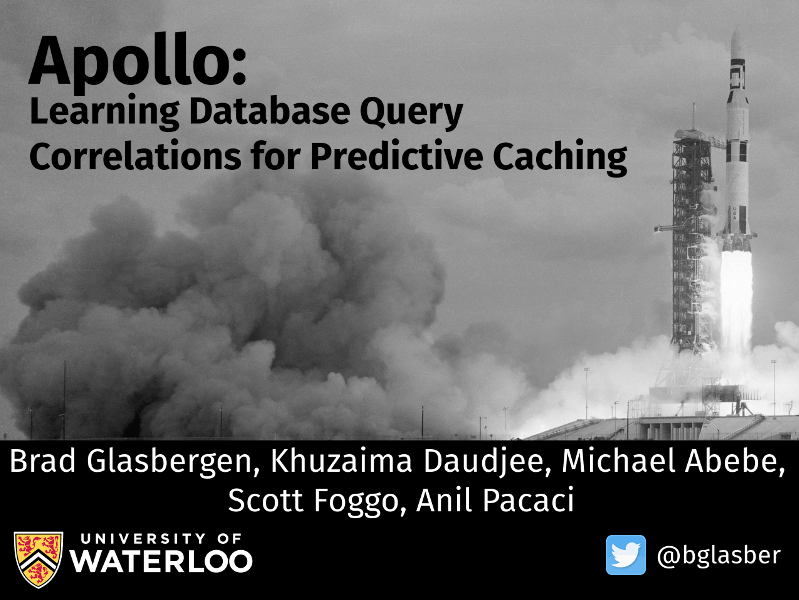
\includegraphics[keepaspectratio=true,width=1.03\paperwidth]{title_slide}
\end{frame}

\begin{frame}{Worldwide Client/Data Center Distribution}
    \begin{figure}
        \center
        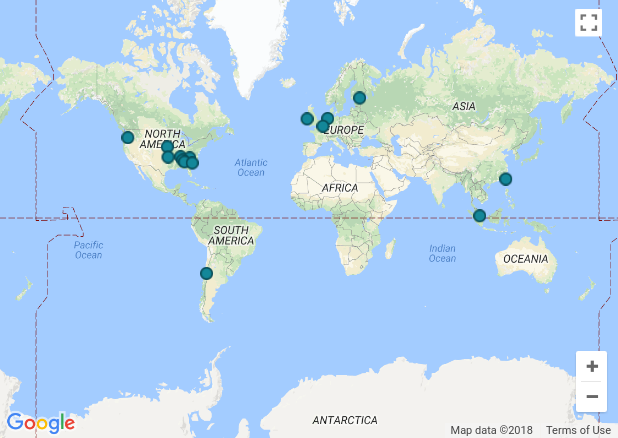
\includegraphics[scale=0.45]{apollo_google_dc}
    \end{figure}
\end{frame}

\begin{frame}{Worldwide Client/Data Center Distribution}
    \begin{figure}
        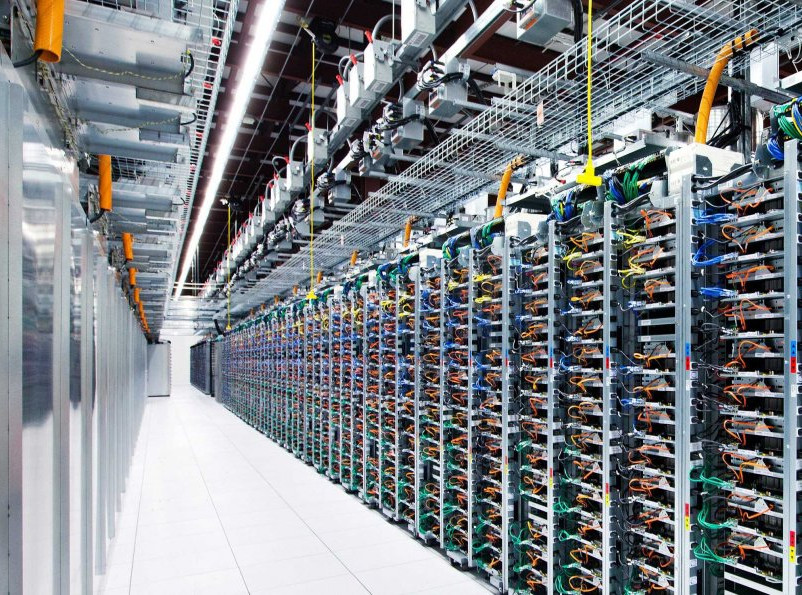
\includegraphics[scale=0.36]{apollo_google_datacenter}
    \end{figure}
\end{frame}

\begin{frame}{Worldwide Client/Data Center Distribution}
    \begin{figure}
        \center
        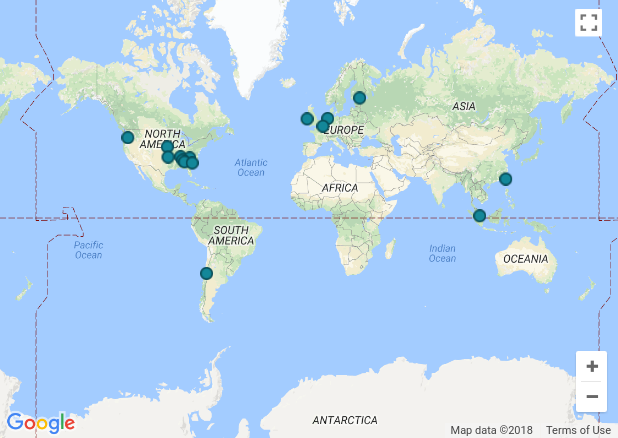
\includegraphics[scale=0.45]{apollo_google_dc}
    \end{figure}
\end{frame}

\begin{frame}{Worldwide Client/Data Center Distribution}
    \begin{figure}
        \center
        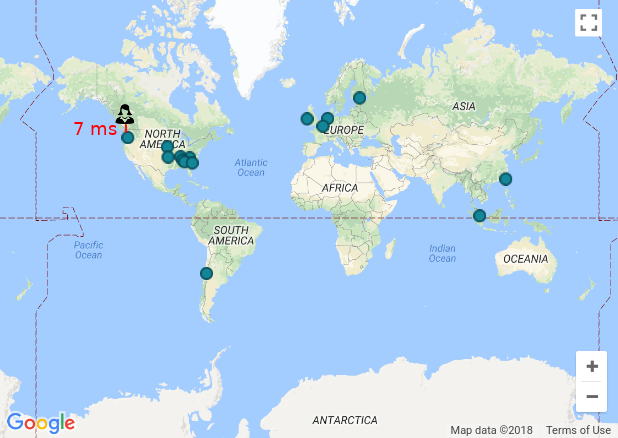
\includegraphics[scale=0.45]{apollo_google_vancouver}
    \end{figure}
\end{frame}

\begin{frame}{Worldwide Client/Data Center Distribution}
    \begin{figure}
        \center
        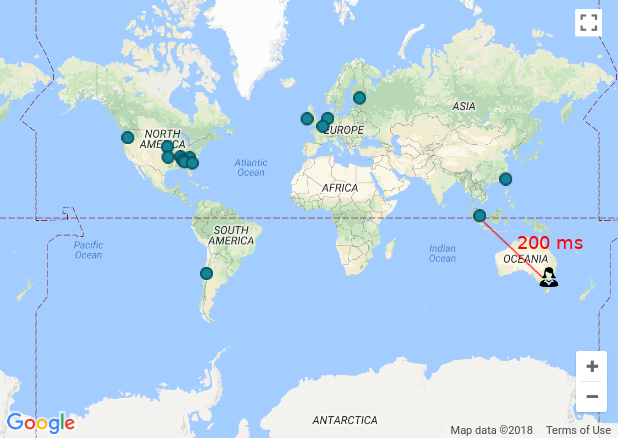
\includegraphics[scale=0.45]{apollo_google_oceania}
    \end{figure}
\end{frame}

\begin{frame}{Latency Effects on Clients}
    \begin{figure}
        \center
        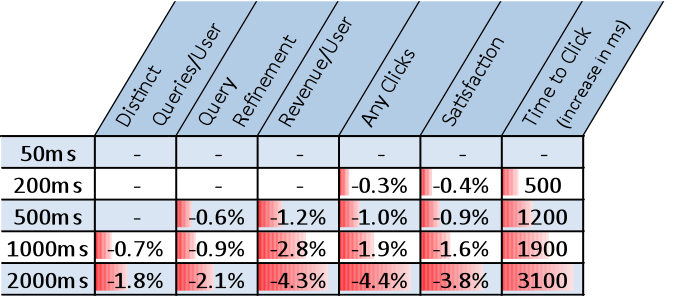
\includegraphics[scale=0.45]{apollo_bing_latency}
    \end{figure}
\end{frame}

\begin{frame}{Edge Nodes}
    \begin{figure}
        \center
        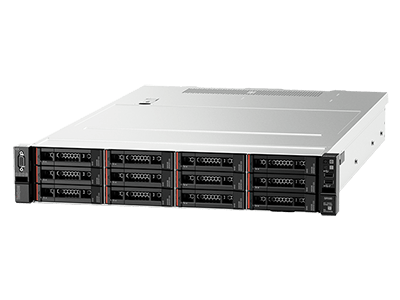
\includegraphics[scale=0.45]{apollo_blade.png}
    \end{figure}
    Company-supplied, ISP hosted servers with limited compute and storage capabilities.
\end{frame}

\begin{frame}{Worldwide Client/Edge Node Distribution}
    \begin{figure}
        \center
        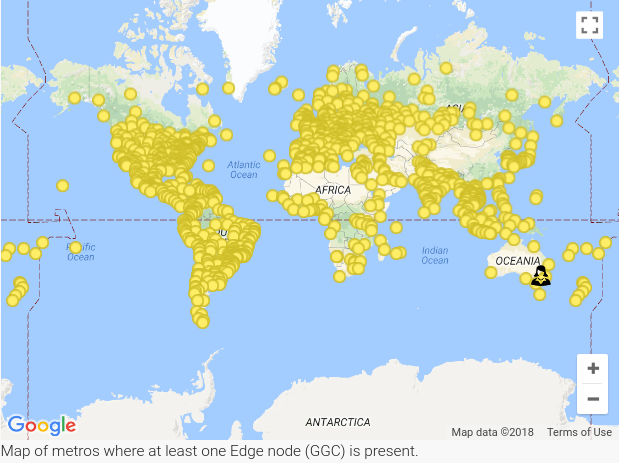
\includegraphics[scale=0.45]{apollo_google_oceania_en}
    \end{figure}
\end{frame}

\begin{frame}{A Solved Problem?}
    \begin{itemize}
        \item{Cache data on edge nodes and reduce latency!}
        \visible<2->{
            \item{{\color{red} Limited storage space for caching!} }
            \item{{\color{red} Data freshness?}}
        }
    \end{itemize}
\end{frame}

\begin{frame}{Amazon Webpage Breakdown}
    \begin{figure}
        \center
        \hspace*{-0.5cm}
        \vspace*{1cm}
        
\includegraphics[scale=0.17]{apollo_amazon_page}
    \end{figure}
\end{frame}

\begin{frame}{Amazon Webpage Breakdown}
    \begin{figure}
        \center
        \hspace*{-0.5cm}
        \vspace*{1cm}
        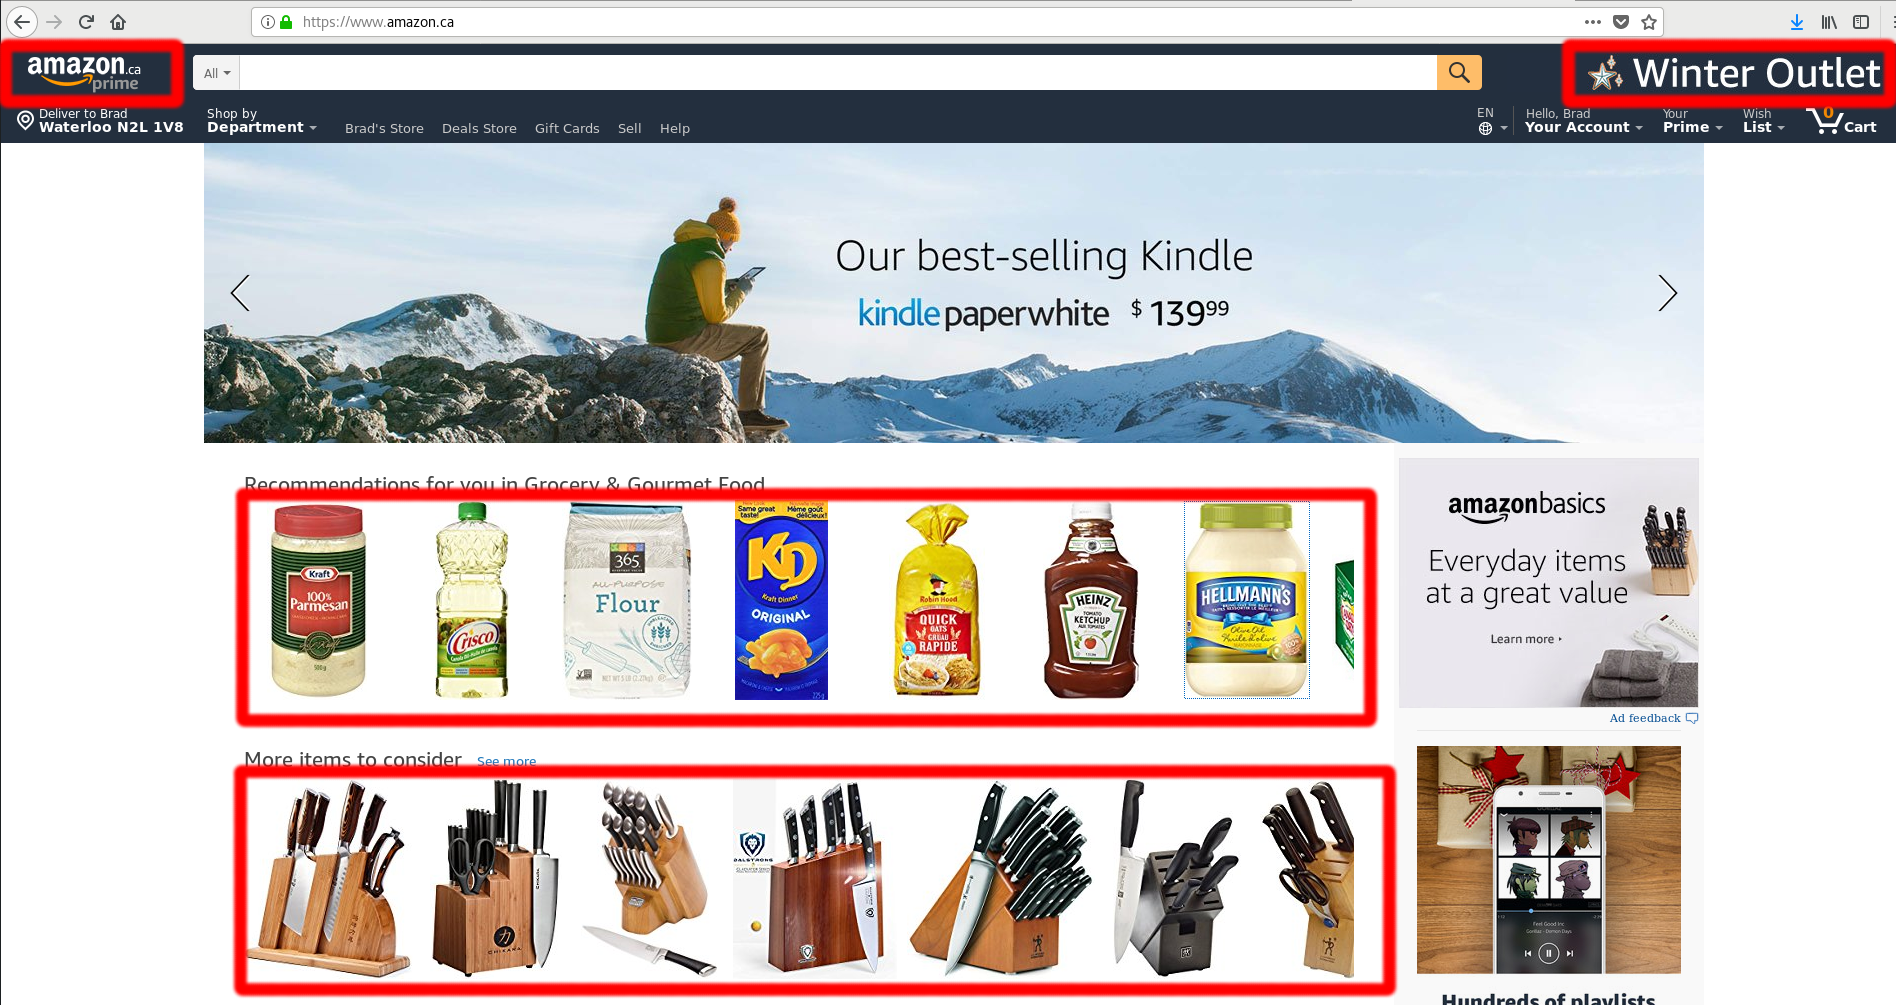
\includegraphics[scale=0.17]{apollo_amazon_static}
    \end{figure}
\end{frame}

\begin{frame}{The State of the Art}
    \begin{itemize}
        \item{Cache \alert{static data} on edge nodes and reduce latency!}
    \end{itemize}
\end{frame}

\begin{frame}{Amazon Webpage Breakdown}
    \begin{figure}
        \center
        \hspace*{-0.5cm}
        \vspace*{1cm}
        
\includegraphics[scale=0.17]{apollo_amazon_page}
    \end{figure}
\end{frame}

\begin{frame}{Amazon --- Dynamic Data}
    \begin{figure}
        \center
        \hspace*{-0.5cm}
        \vspace*{1cm}
        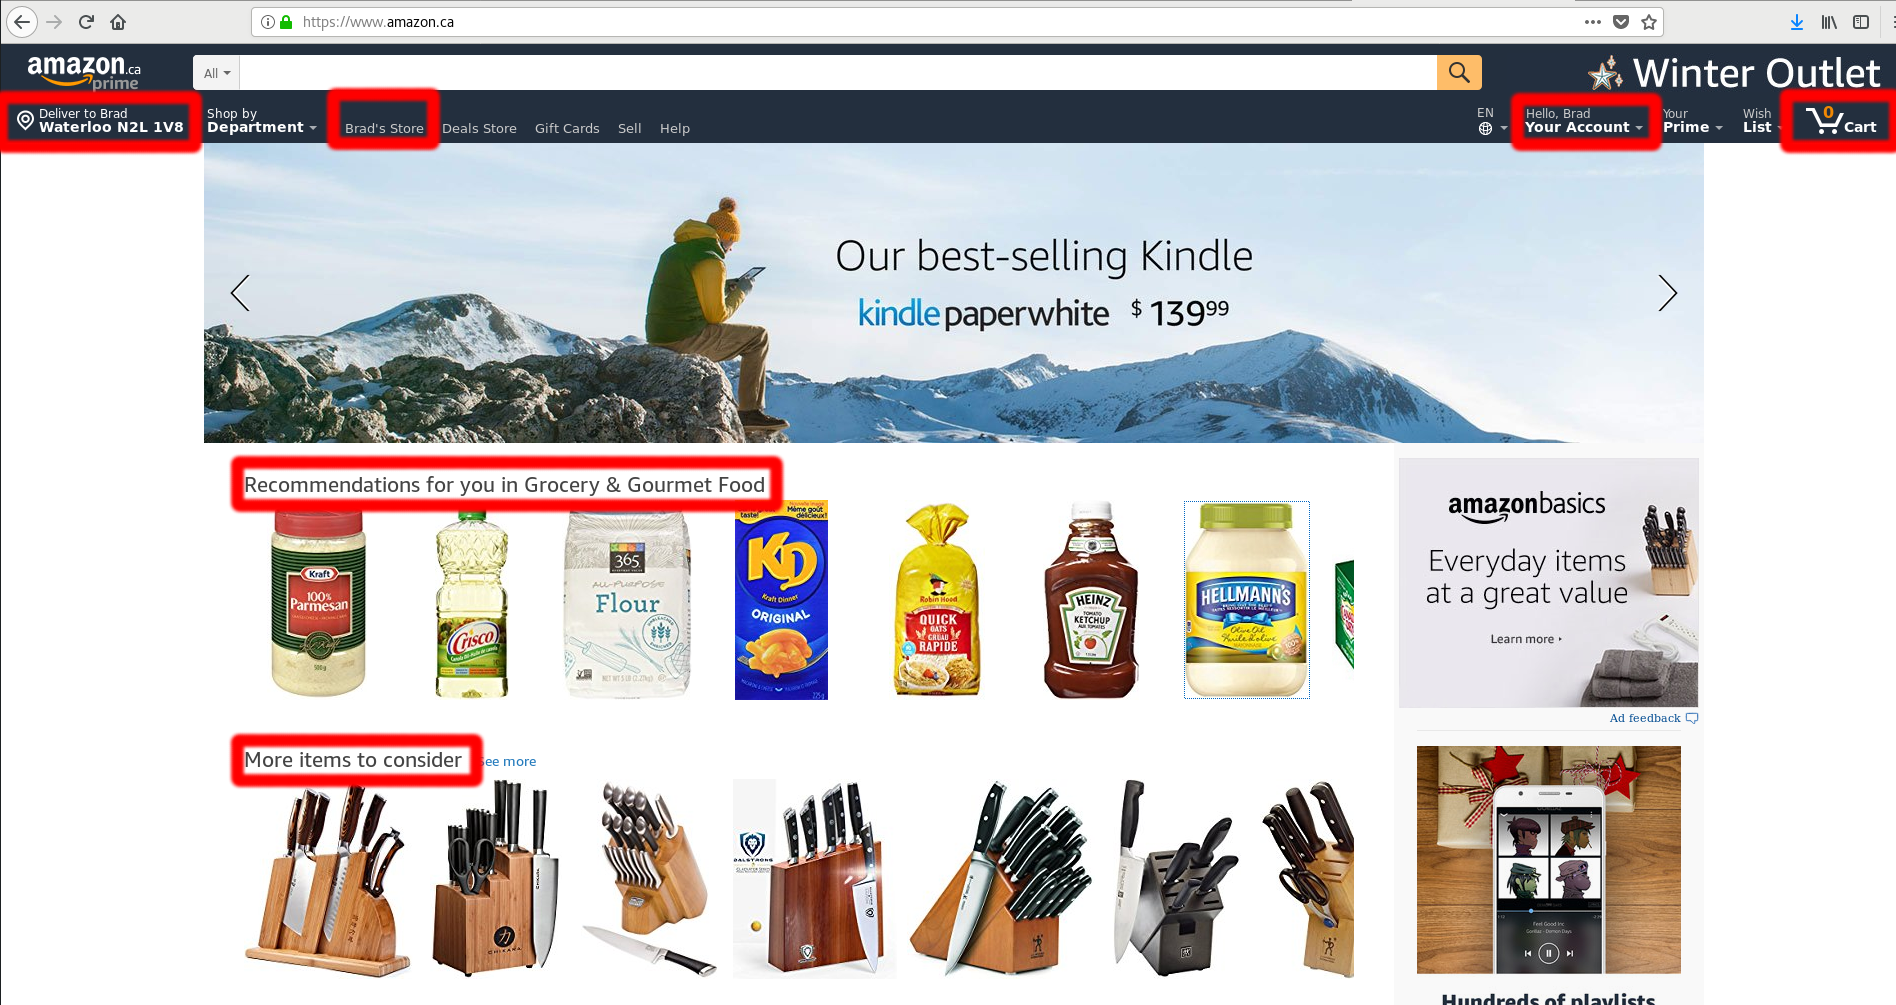
\includegraphics[scale=0.17]{apollo_amazon_dynamic}
    \end{figure}
\end{frame}

\begin{frame}[fragile]{Dynamic Data Requests}
        \begin{lstlisting}[
                   language=SQL,
                   basicstyle=\ttfamily,
                   commentstyle=\color{gray},
                   escapeinside={(*@}{@*)},
                ]
1. SELECT (*@ \cfbox{red}{C\_ID} @*) FROM CUSTOMER WHERE 
C_UNAME = @C_UN and C_PASSWD = @C_PAS

2. SELECT MAX(O_ID) FROM ORDERS WHERE
O_C_ID = (*@ \cfbox{red}{@C\_ID} @*)
        \end{lstlisting}
\end{frame}

\begin{frame}{Query Patterns}
    Execution of a query informs which queries will execute next, and
    with what parameters.
\end{frame}

\begin{frame}[fragile]{Dynamic Data Requests}
        \begin{lstlisting}[
                   language=SQL,
                   basicstyle=\ttfamily,
                   commentstyle=\color{gray},
                   escapeinside={(*@}{@*)},
                ]
1. SELECT (*@ \cfbox{red}{C\_ID} @*) FROM CUSTOMER WHERE 
C_UNAME = @C_UN and C_PASSWD = @C_PAS

2. SELECT MAX(O_ID) FROM ORDERS WHERE
O_C_ID = (*@ \cfbox{red}{@C\_ID} @*)
        \end{lstlisting}
\end{frame}

\begin{frame}{Predictive Caching}
    \begin{figure}
        \center
        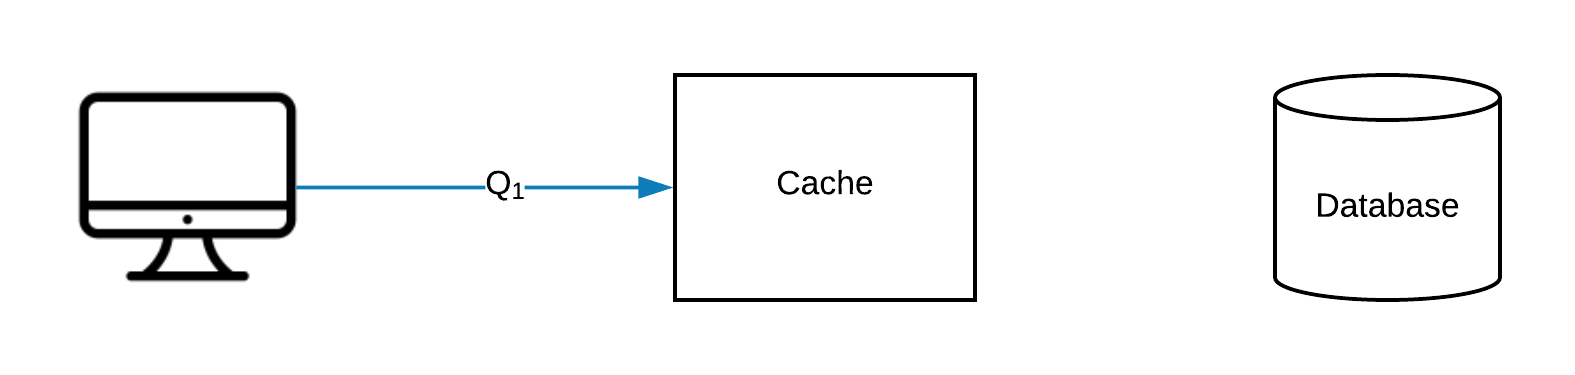
\includegraphics[scale=0.17]{apollo_predictive_execution}
    \end{figure}
\end{frame}

\begin{frame}{Predictive Caching}
    \begin{figure}
        \center
        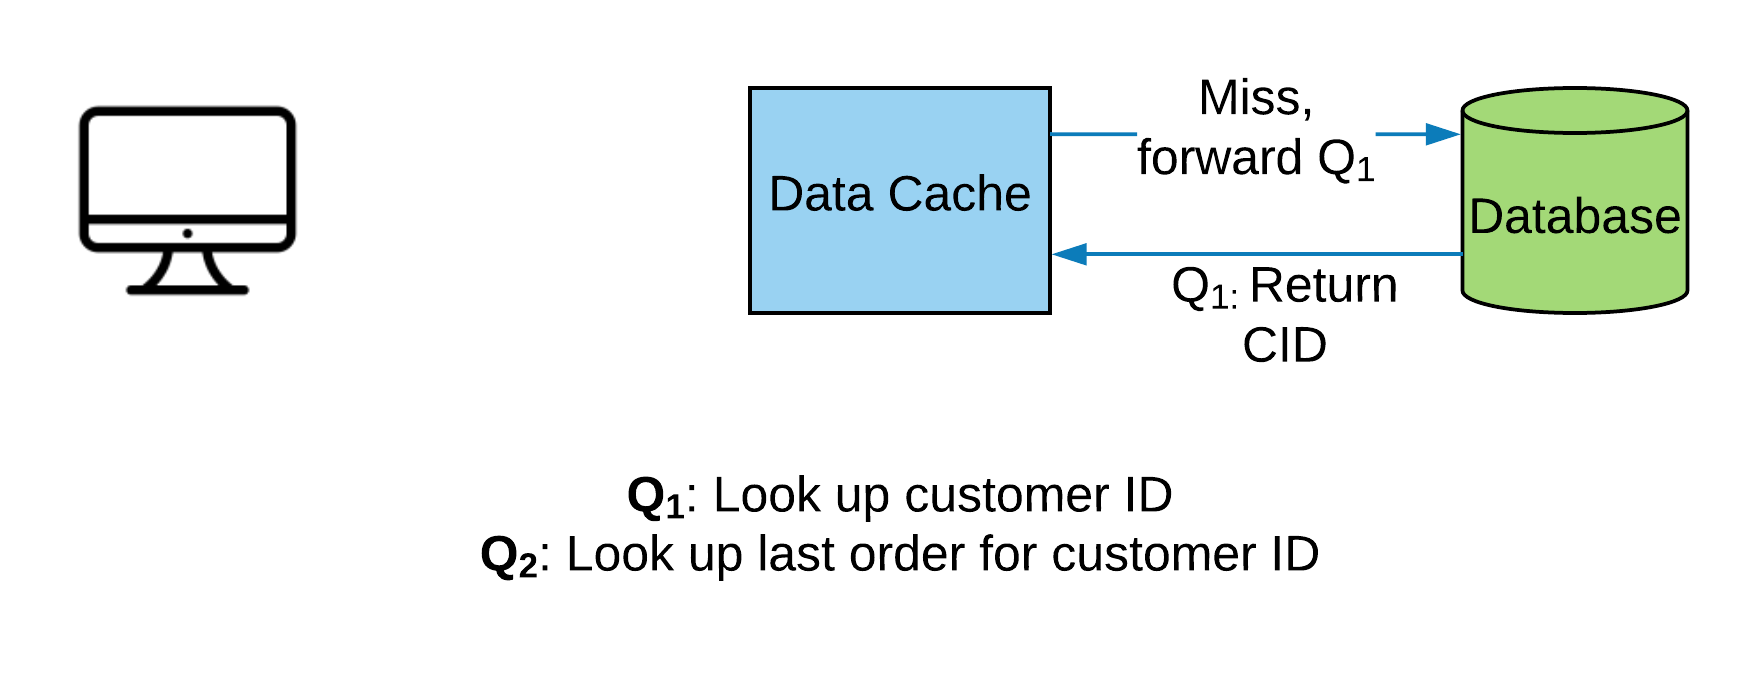
\includegraphics[scale=0.17]{apollo_predictive_execution_2}
    \end{figure}
\end{frame}

\begin{frame}{Predictive Caching}
    \begin{figure}
        \center
        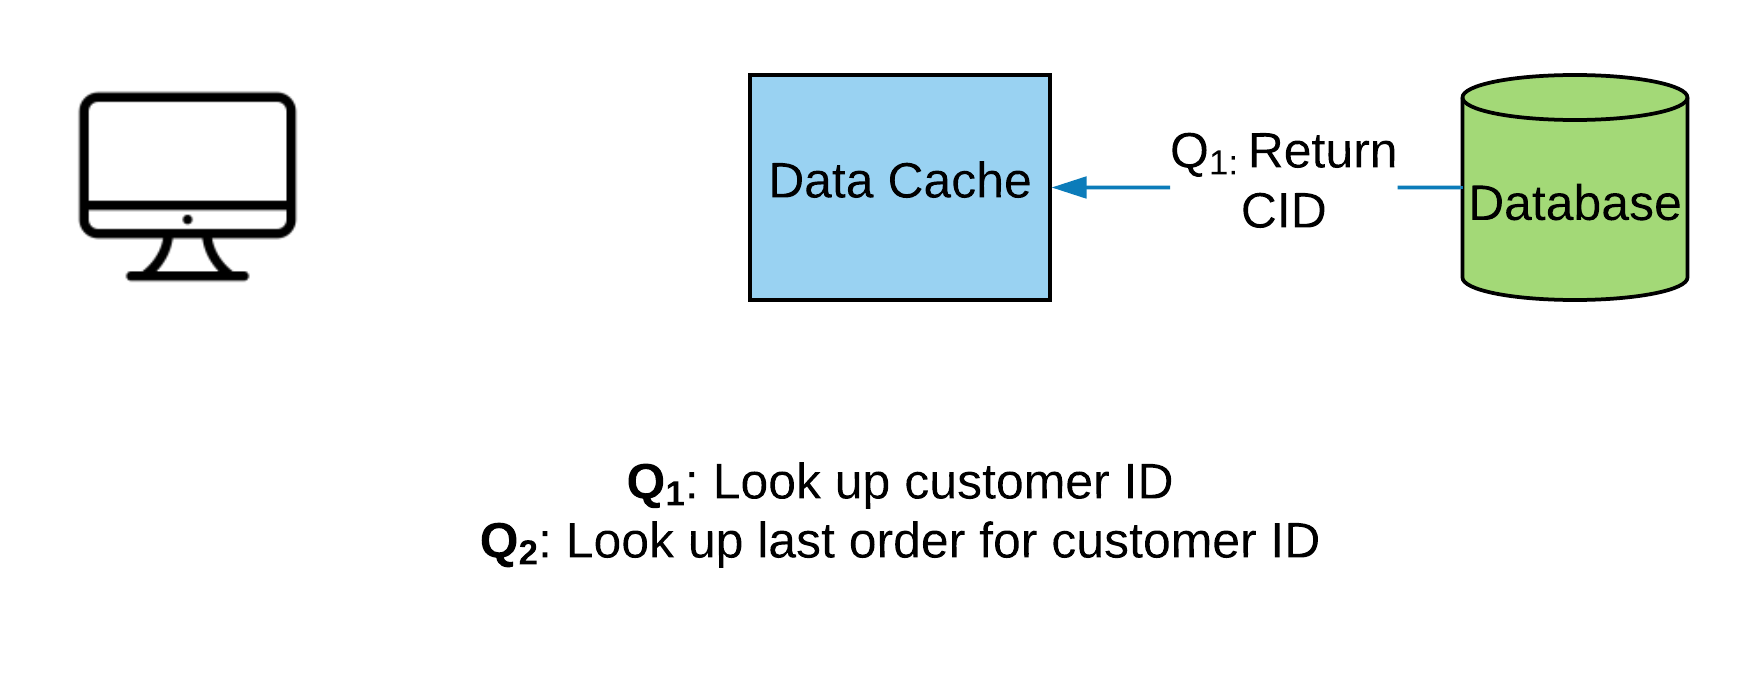
\includegraphics[scale=0.17]{apollo_predictive_execution_3}
    \end{figure}
\end{frame}

\begin{frame}{Predictive Caching}
    \begin{figure}
        \center
        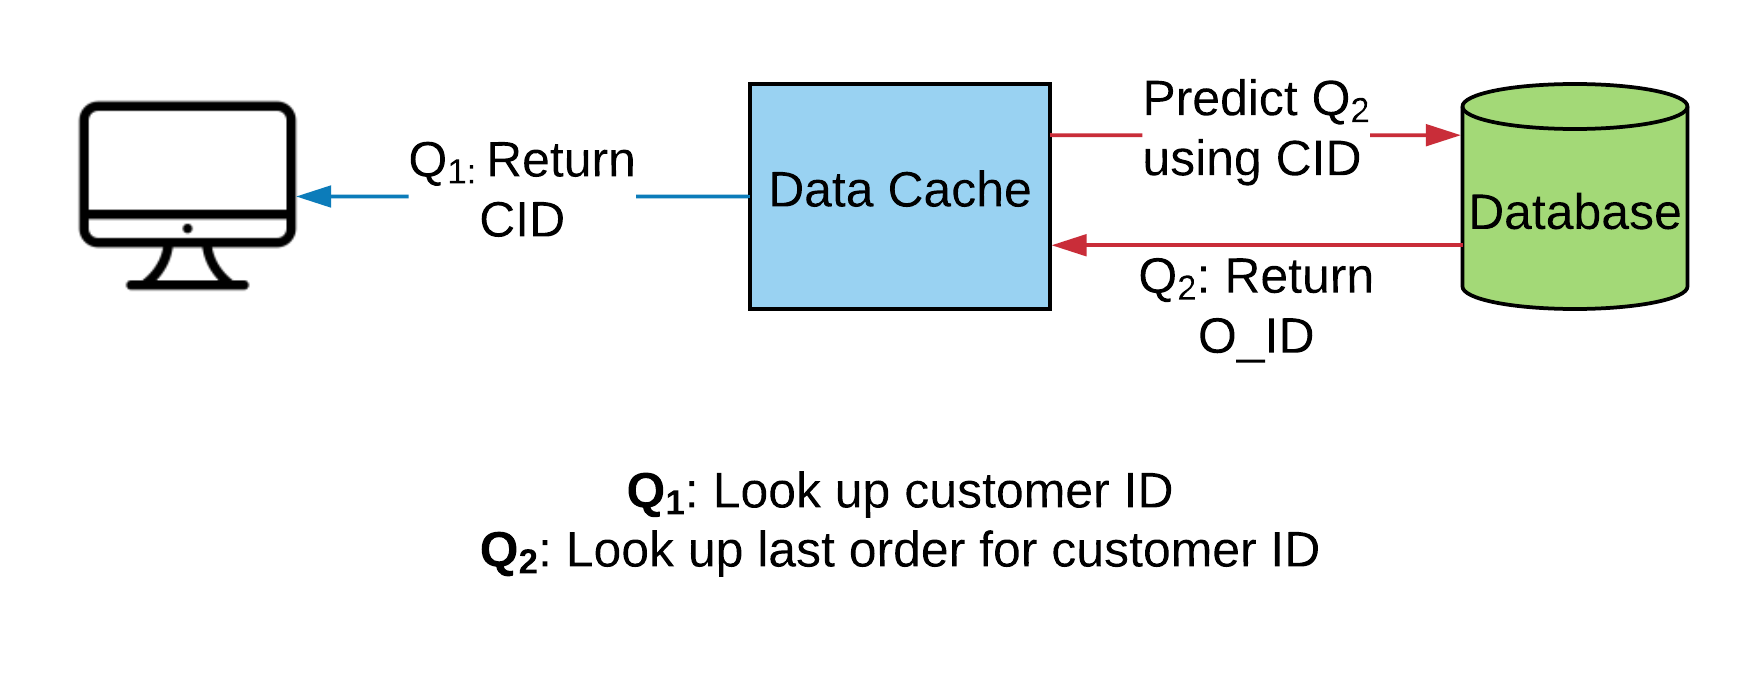
\includegraphics[scale=0.17]{apollo_predictive_execution_4}
    \end{figure}
\end{frame}

\begin{frame}{Apollo: Caching Dynamic Data on a Global Scale}
    Requirements:
    \begin{itemize}
        \visible<2->{
            \item{Adaptive method to cache based on client behaviour patterns}
        }
        \visible<3->{
            \item{Computationally efficient means of managing updates to cached data}
        }
    \end{itemize}
\end{frame}

\begin{frame}{Table of contents}
  \setbeamertemplate{section in toc}[sections numbered]
  \tableofcontents[hideallsubsections]
\end{frame}

\section{Predictive Query Model}

\begin{frame}[fragile]{A Query Submission}
    \begin{center}
SELECT \cfbox{red}{C\_ID} FROM CUSTOMER WHERE
C\_UNAME = 'Alice' and C\_PASSWD = 'pass'

SELECT MAX(O\_ID) FROM ORDERS WHERE
O\_C\_ID = \cfbox{red}{3}
    \end{center}
\end{frame}

\begin{frame}[fragile]{Abstracting to Query Templates}
    \begin{center}
SELECT \cfbox{red}{C\_ID} FROM CUSTOMER WHERE
C\_UNAME = \textbf{?} and C\_PASSWD = \textbf{?}

SELECT MAX(O\_ID) FROM ORDERS WHERE
O\_C\_ID = \cfbox{red}{\textbf{?}}
    \end{center}
\end{frame}

\begin{frame}[fragile]{Client Query Streams}
    \begin{figure}
        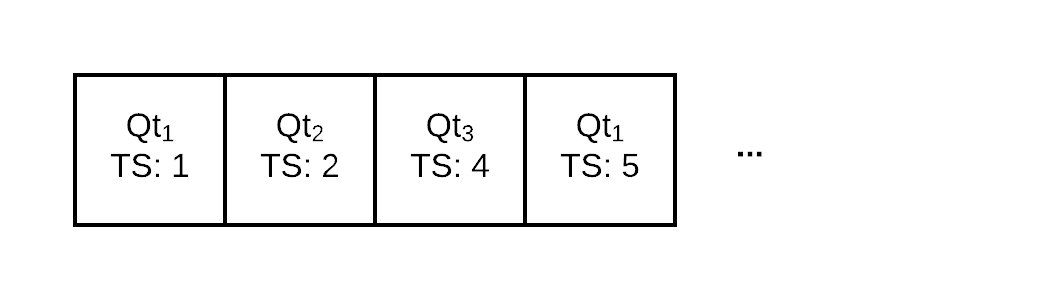
\includegraphics[scale=0.2]{apollo_client_query_stream}
    \end{figure}
\end{frame}

\begin{frame}[fragile]{Client Query Streams}
    \begin{figure}
        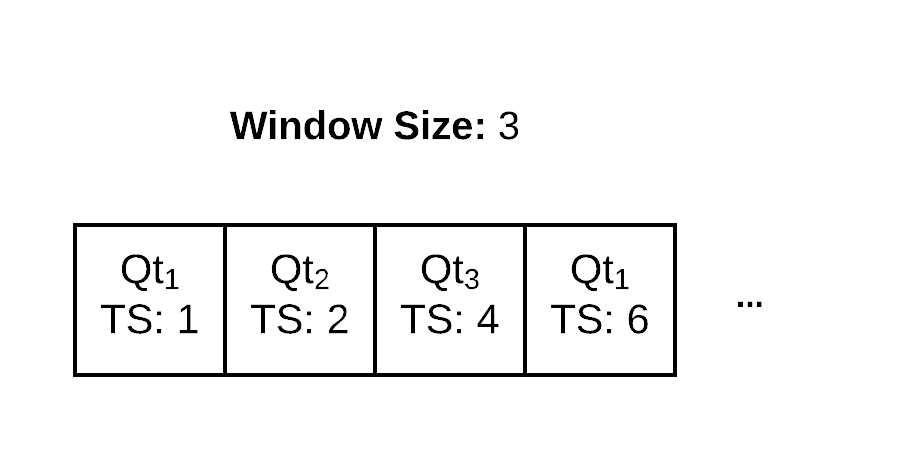
\includegraphics[scale=0.2]{apollo_client_query_stream_2}
    \end{figure}
\end{frame}

\begin{frame}[fragile]{Client Query Streams}
    \begin{figure}
        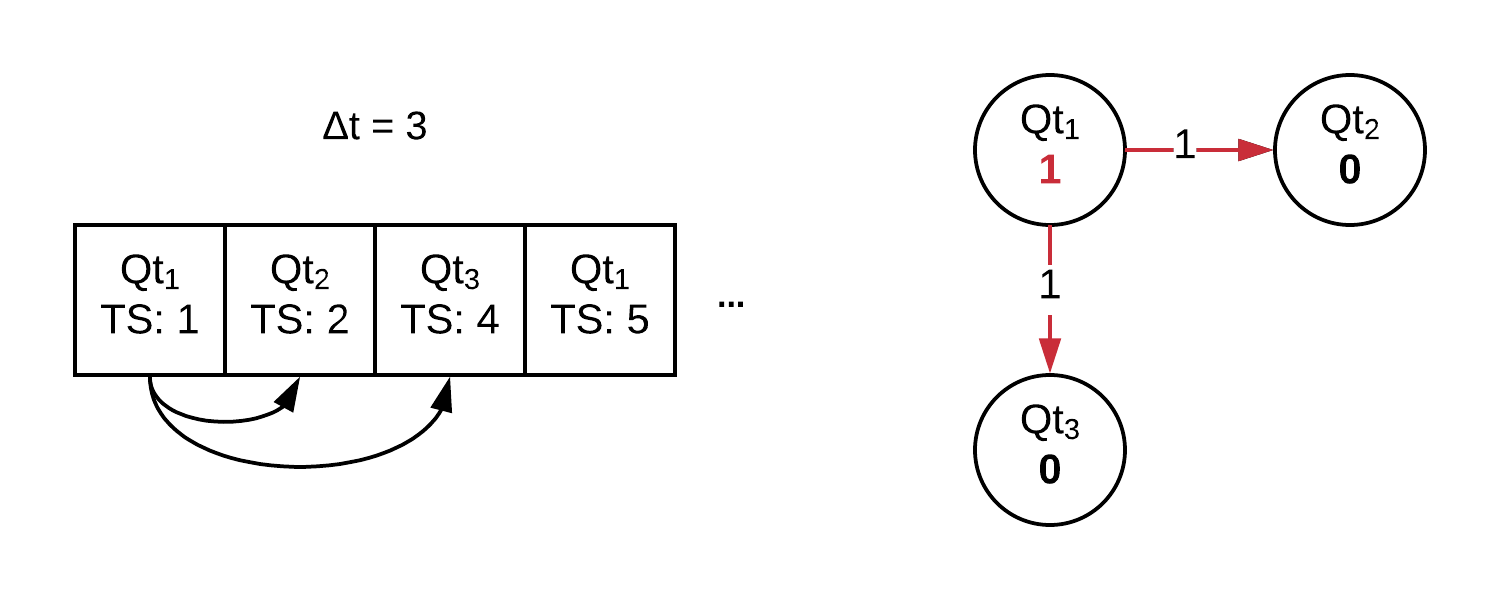
\includegraphics[scale=0.2]{apollo_client_query_stream_3}
    \end{figure}
\end{frame}

\begin{frame}[fragile]{Client Query Streams}
    \begin{figure}
        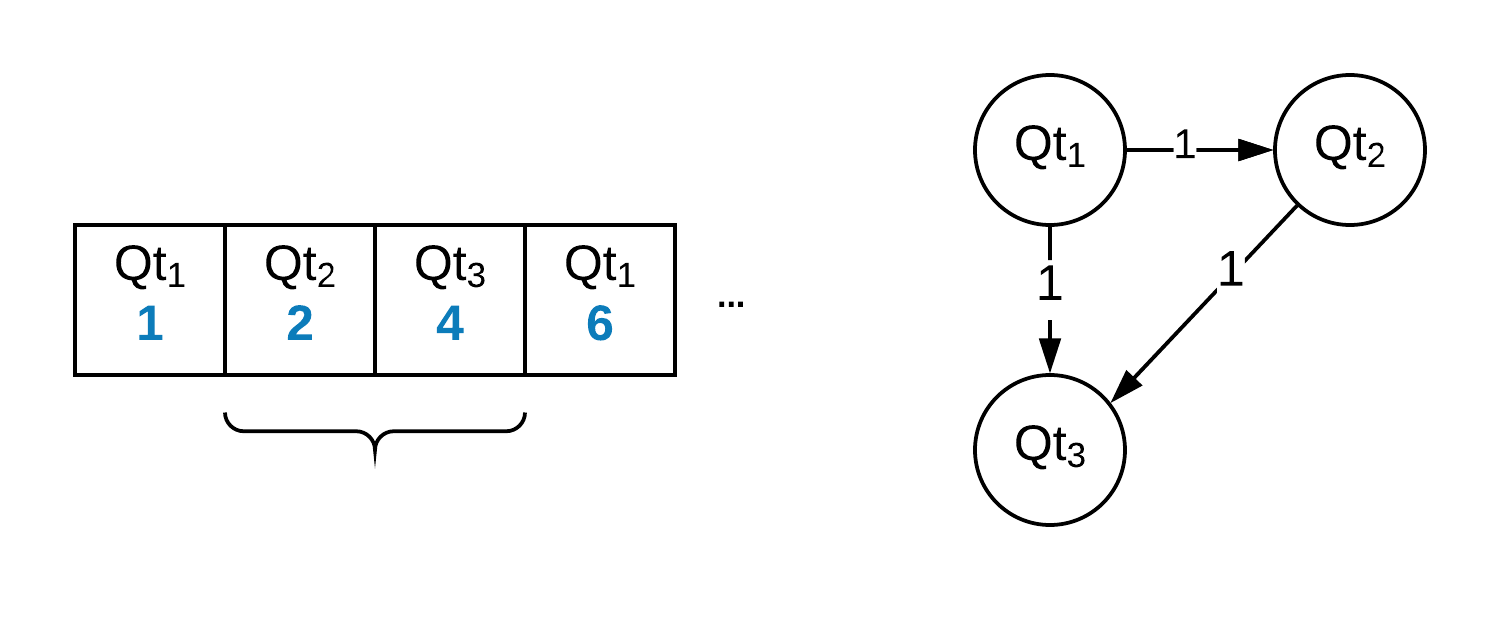
\includegraphics[scale=0.2]{apollo_client_query_stream_4}
    \end{figure}
\end{frame}

\begin{frame}[fragile]{Client Query Streams}
    \begin{figure}
        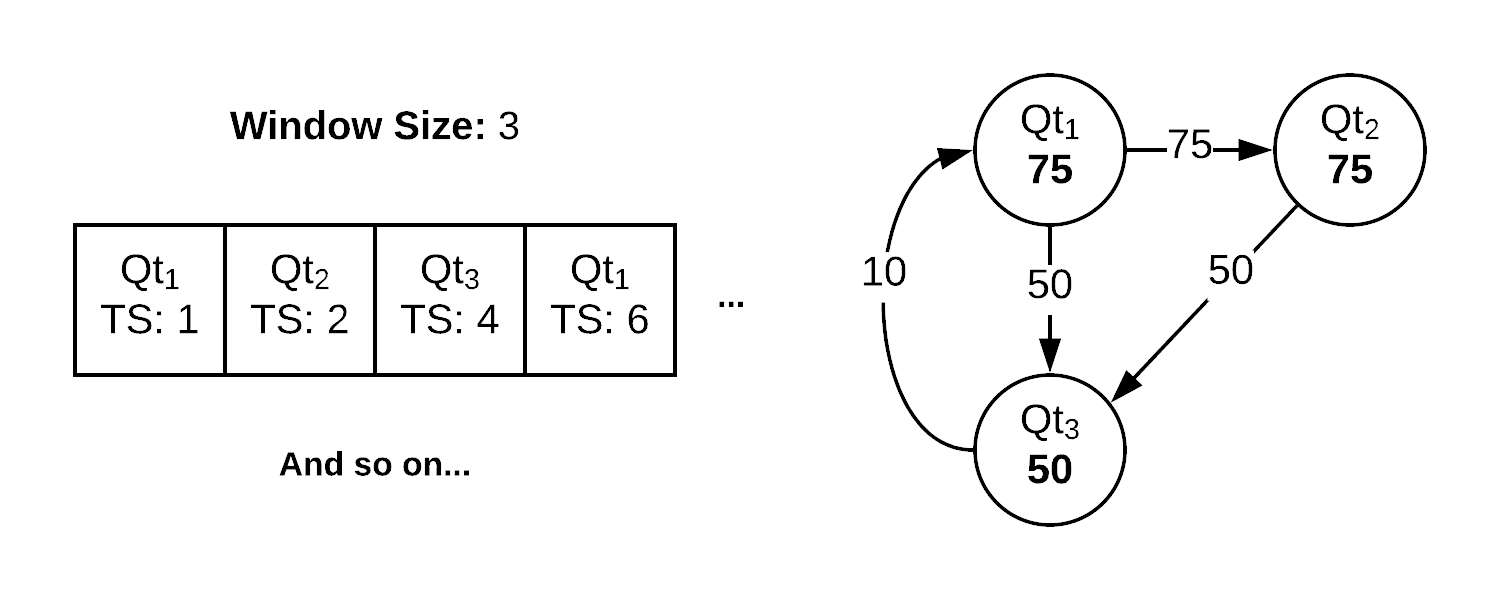
\includegraphics[scale=0.2]{apollo_client_query_stream_5}
    \end{figure}
\end{frame}

\begin{frame}[fragile]{Query Transition Graph}
    \begin{figure}
        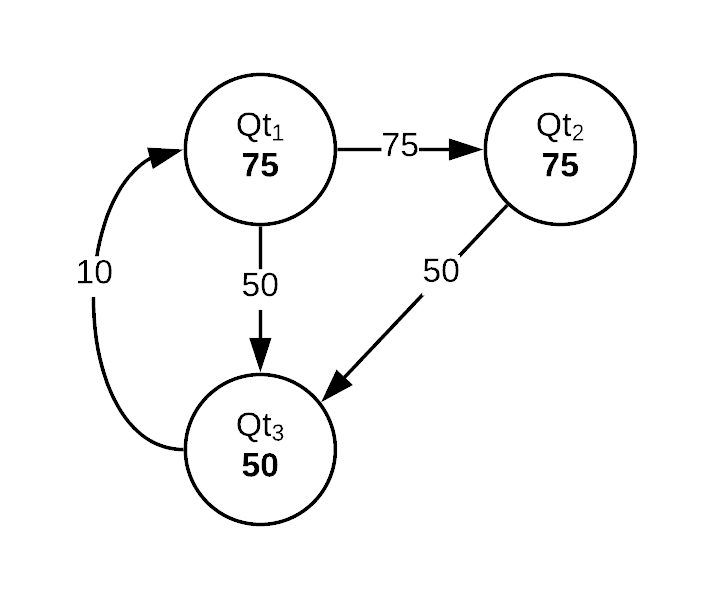
\includegraphics[scale=0.2]{apollo_transition_graph}
    \end{figure}
    \visible<2->{
        $P(Qt_{2}|Qt_{1};T\leq\Delta t) = \frac{75}{75} = 1$\\
    }
    \visible<3->{
        $P(Qt_{3}|Qt_{1};T\leq\Delta t) = \frac{10}{50} = \frac{1}{5}$
    }
\end{frame}

\begin{frame}[fragile]{Query Transition Graph}
    The query transition graphs tells us:
    \begin{itemize}
        \item{How often a query template is executed}
        \visible<2->{
        \item{Which query templates are \alert{correlated} with each other}
        }
    \end{itemize}
    \visible<3->{
        { \color{red} Need parameter mappings for predictive caching!}
    }
\end{frame}

\begin{frame}[fragile]{Client Query Streams}
    \begin{figure}
        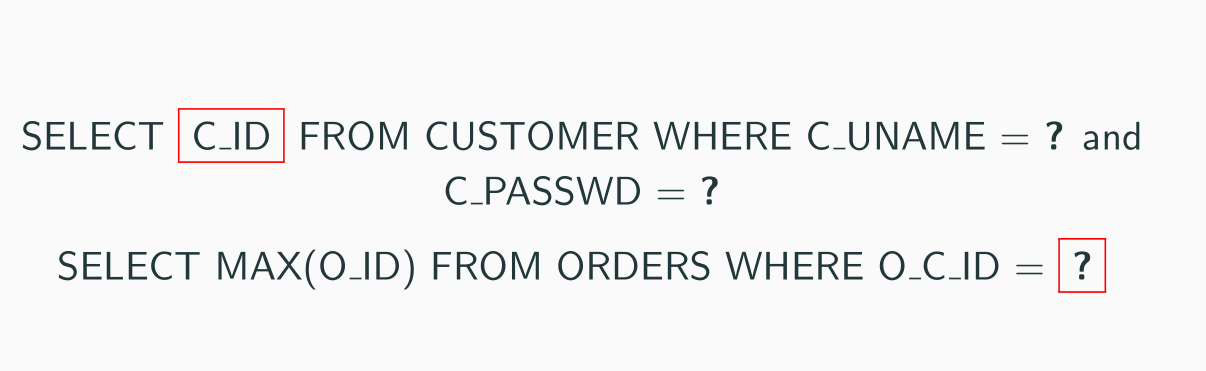
\includegraphics[scale=0.25]{apollo_parameter_mappings}
    \end{figure}
\end{frame}

\begin{frame}[fragile]{Client Query Streams}
    \begin{figure}
        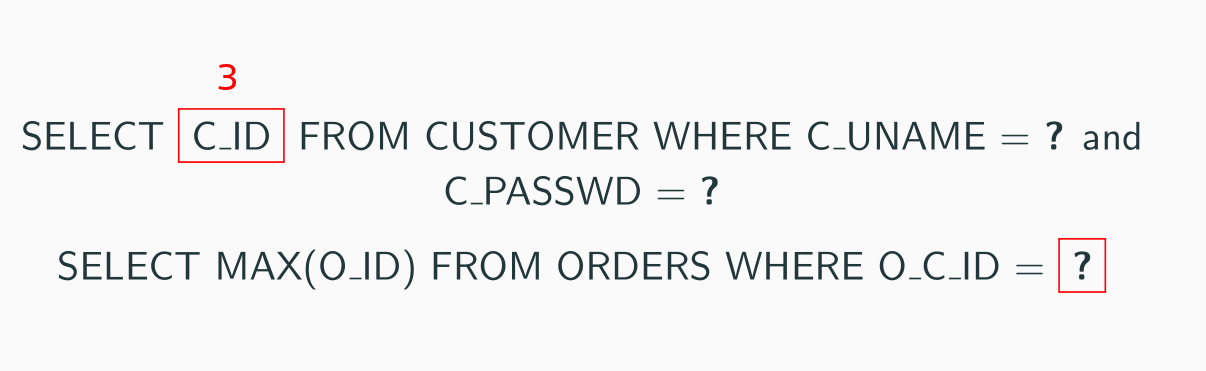
\includegraphics[scale=0.25]{apollo_parameter_mappings_2}
    \end{figure}
\end{frame}

\begin{frame}[fragile]{Client Query Streams}
    \begin{figure}
        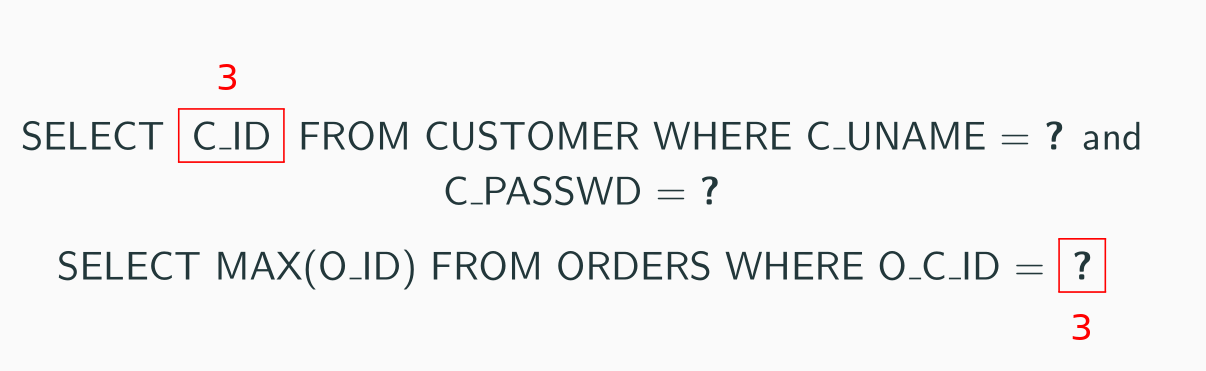
\includegraphics[scale=0.25]{apollo_parameter_mappings_3}
    \end{figure}
\end{frame}

\begin{frame}[fragile]{Client Query Streams}
    \begin{figure}
        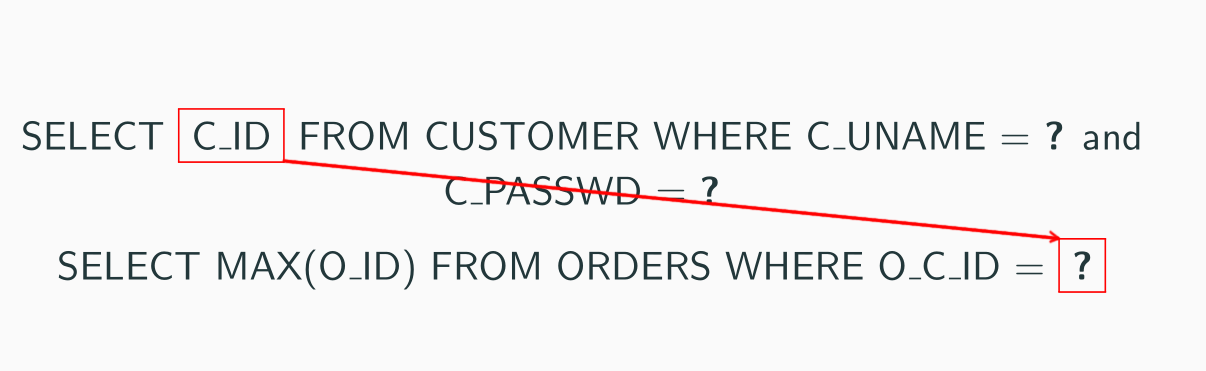
\includegraphics[scale=0.25]{apollo_parameter_mappings_4}
    \end{figure}
\end{frame}

\begin{frame}[fragile]{Pipelining Query Predictions}
    \begin{figure}
        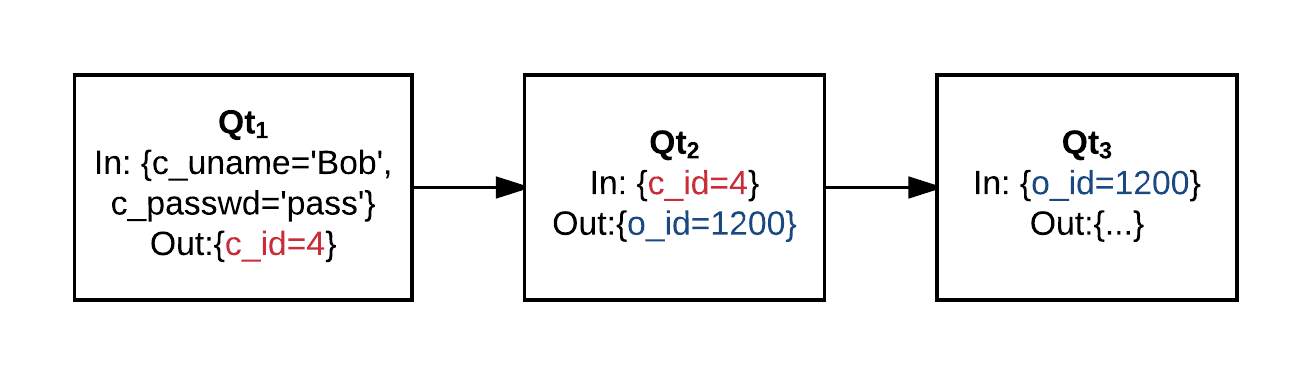
\includegraphics[scale=0.22]{apollo_query_pipeline}
    \end{figure}
\end{frame}

\begin{frame}[fragile]{Formalizing...}
A \alert{fully defined query template} (FDQ) $\mathit{Qt}_j$ has all of its inputs provided
by some set, possibly empty, of prior query templates $\mathit{Qt_i}_1, \mathit{Qt_i}_2, \ldots, \mathit{Qt_i}_m$,
where each $\mathit{Qt_i}_k, \forall k \in [1,m]$, is a fully defined query template.
\end{frame}

\begin{frame}[fragile]{Example FDQs}
    \begin{figure}
        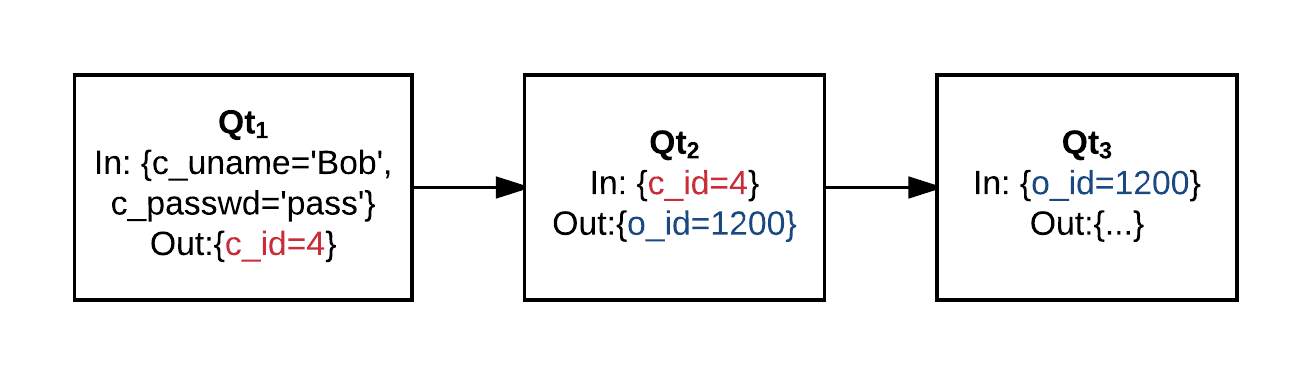
\includegraphics[scale=0.22]{apollo_query_pipeline}
    \end{figure}
    \visible<2->{
        $\mathit{Qt}_2$ and $\mathit{Qt}_3$ are FDQs.\\
    }
    \visible<3->{
        $\mathit{Qt}_1$ is a dependency query of $\mathit{Qt}_2$.\\
        $\mathit{Qt}_2$ is a dependency query of $\mathit{Qt}_3$.\\
    }
    \visible<4->{
        FDQs and their dependency queries form the \alert{dependency graph}.
    }
\end{frame}

\begin{frame}[fragile]{Core Prediction Routine}
    \begin{figure}
        \hspace*{-1cm}
        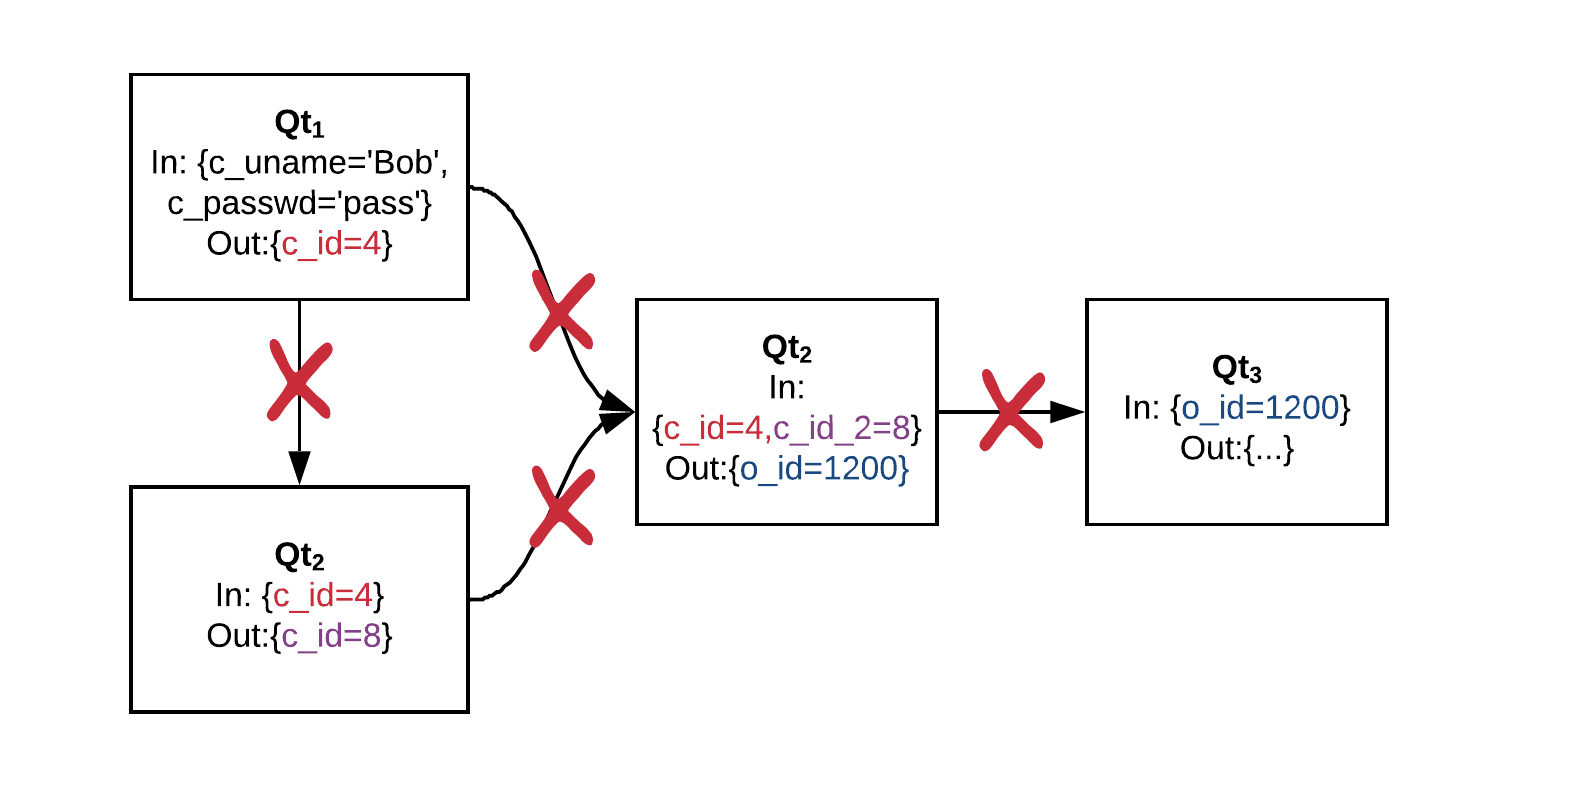
\includegraphics[scale=0.22]{apollo_cpr}
    \end{figure}
\end{frame}

\begin{frame}[fragile]{Core Prediction Routine}
    \begin{figure}
        \hspace*{-1cm}
        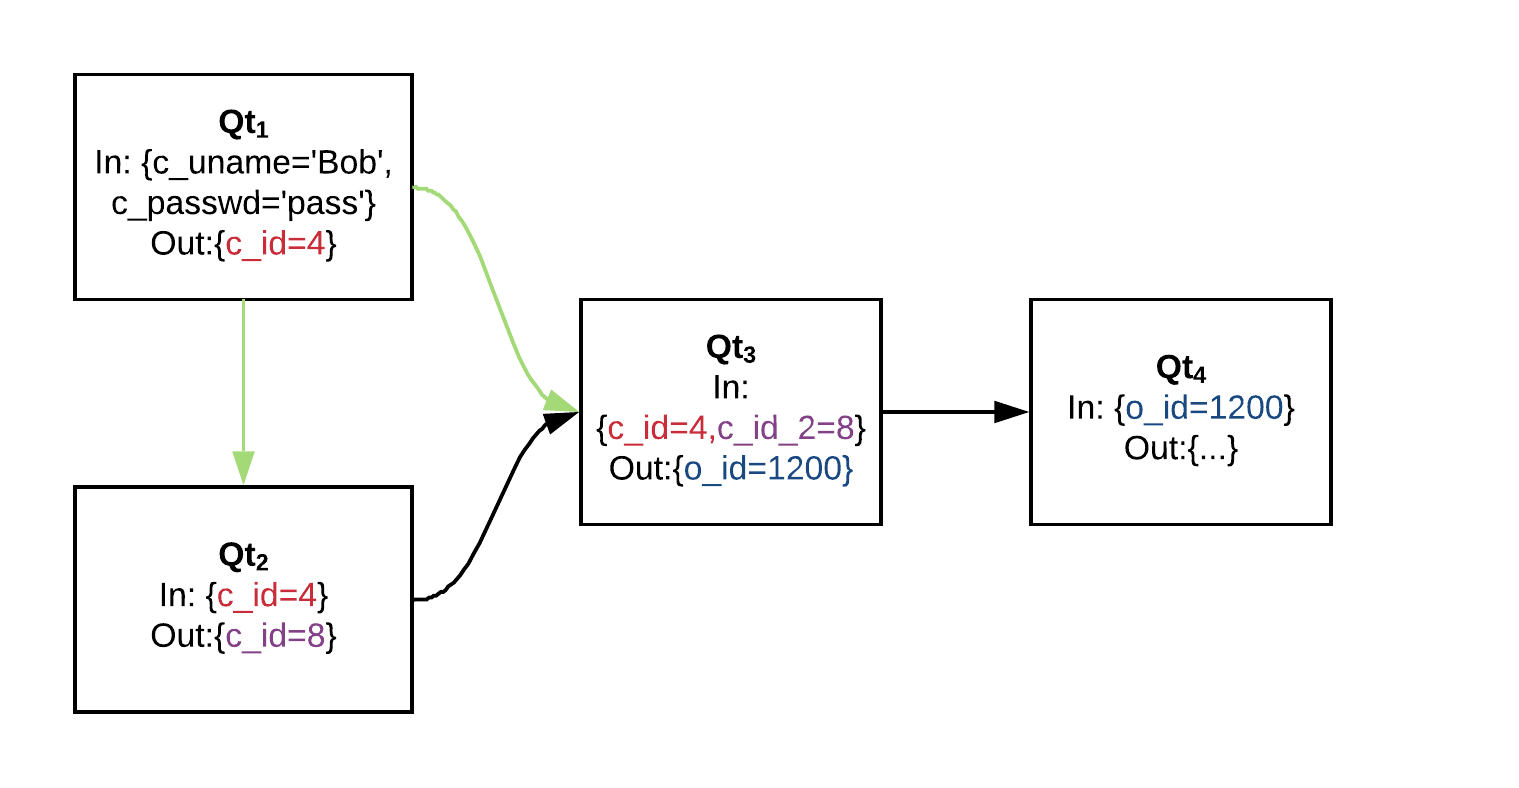
\includegraphics[scale=0.22]{apollo_cpr_2}
    \end{figure}
\end{frame}

\begin{frame}[fragile]{Core Prediction Routine}
    \begin{figure}
        \hspace*{-1cm}
        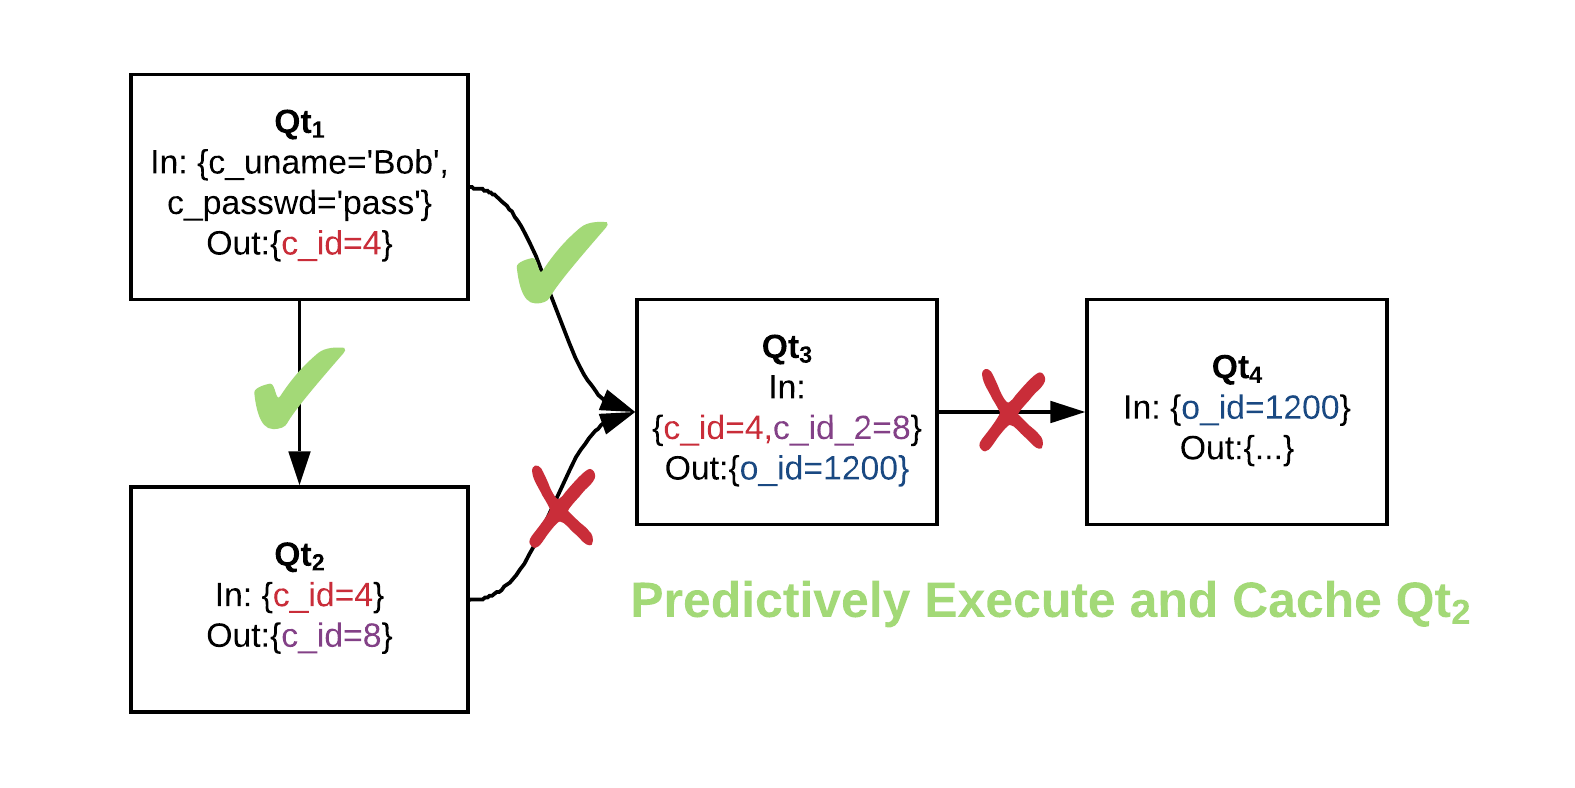
\includegraphics[scale=0.22]{apollo_cpr_3}
    \end{figure}
\end{frame}

\begin{frame}[fragile]{Core Prediction Routine}
    \begin{figure}
        \hspace*{-1cm}
        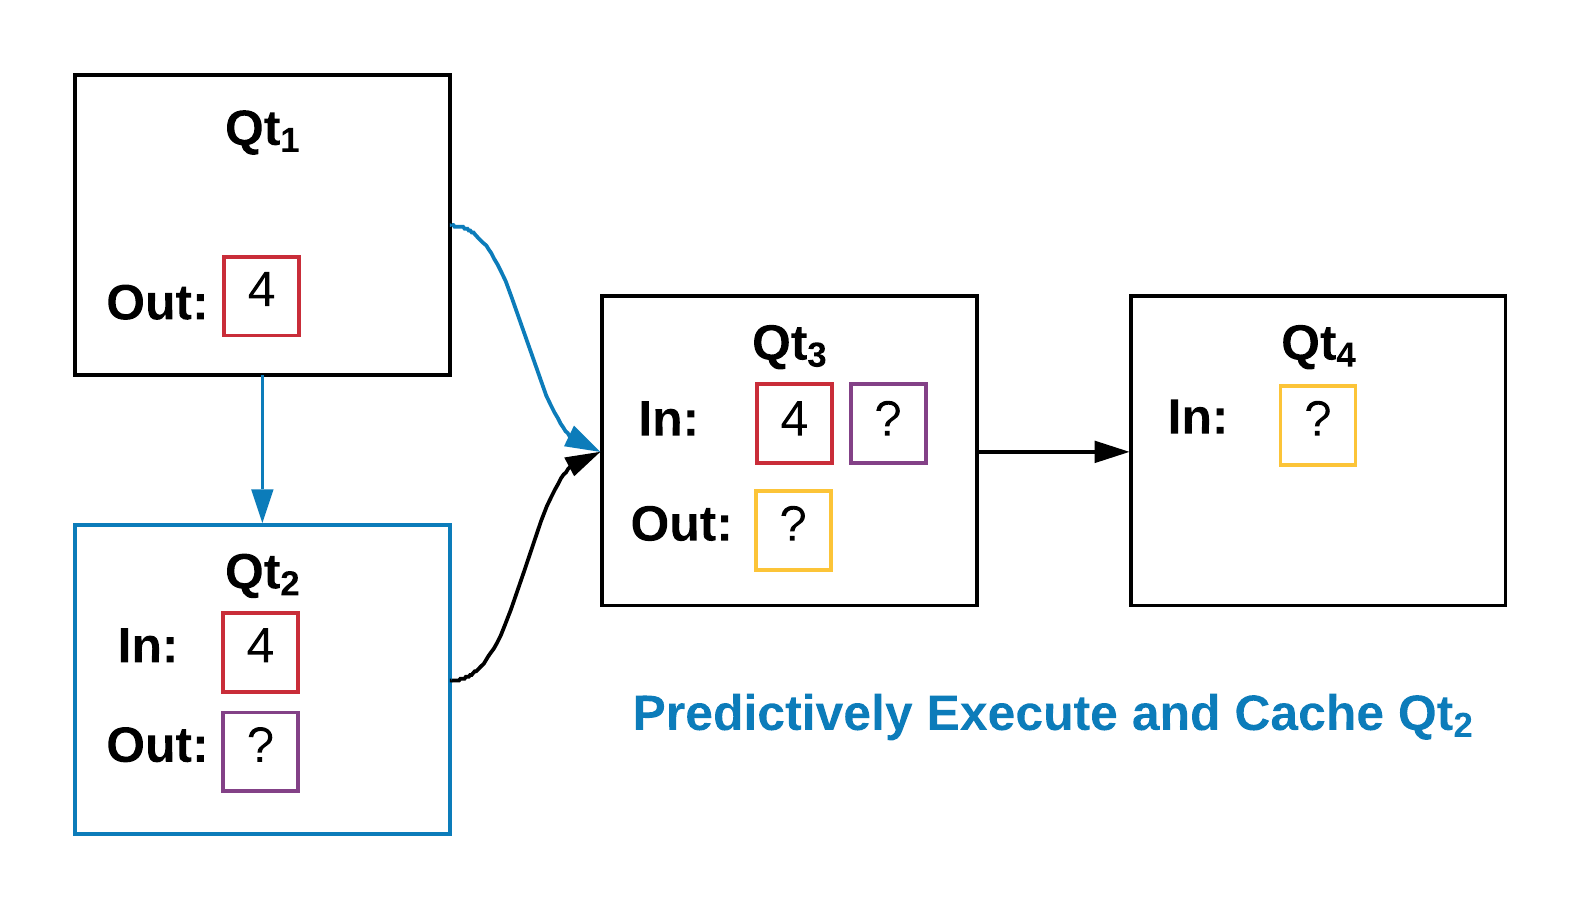
\includegraphics[scale=0.22]{apollo_cpr_4}
    \end{figure}
\end{frame}

\begin{frame}[fragile]{Core Prediction Routine}
    \begin{figure}
        \hspace*{-1cm}
        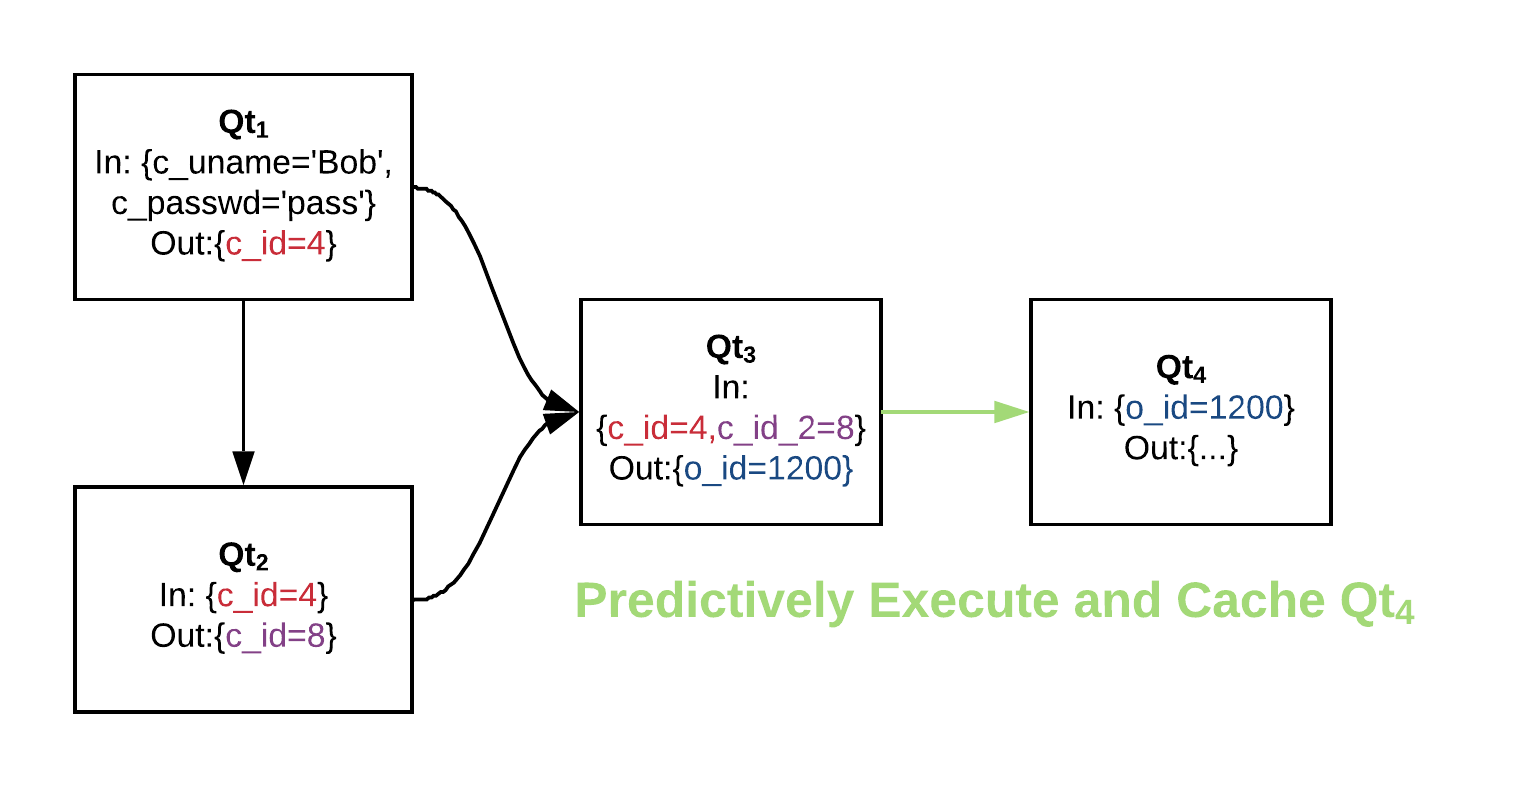
\includegraphics[scale=0.22]{apollo_cpr_5}
    \end{figure}
\end{frame}

\begin{frame}[fragile]{Core Prediction Routine}
    \begin{figure}
        \hspace*{-1cm}
        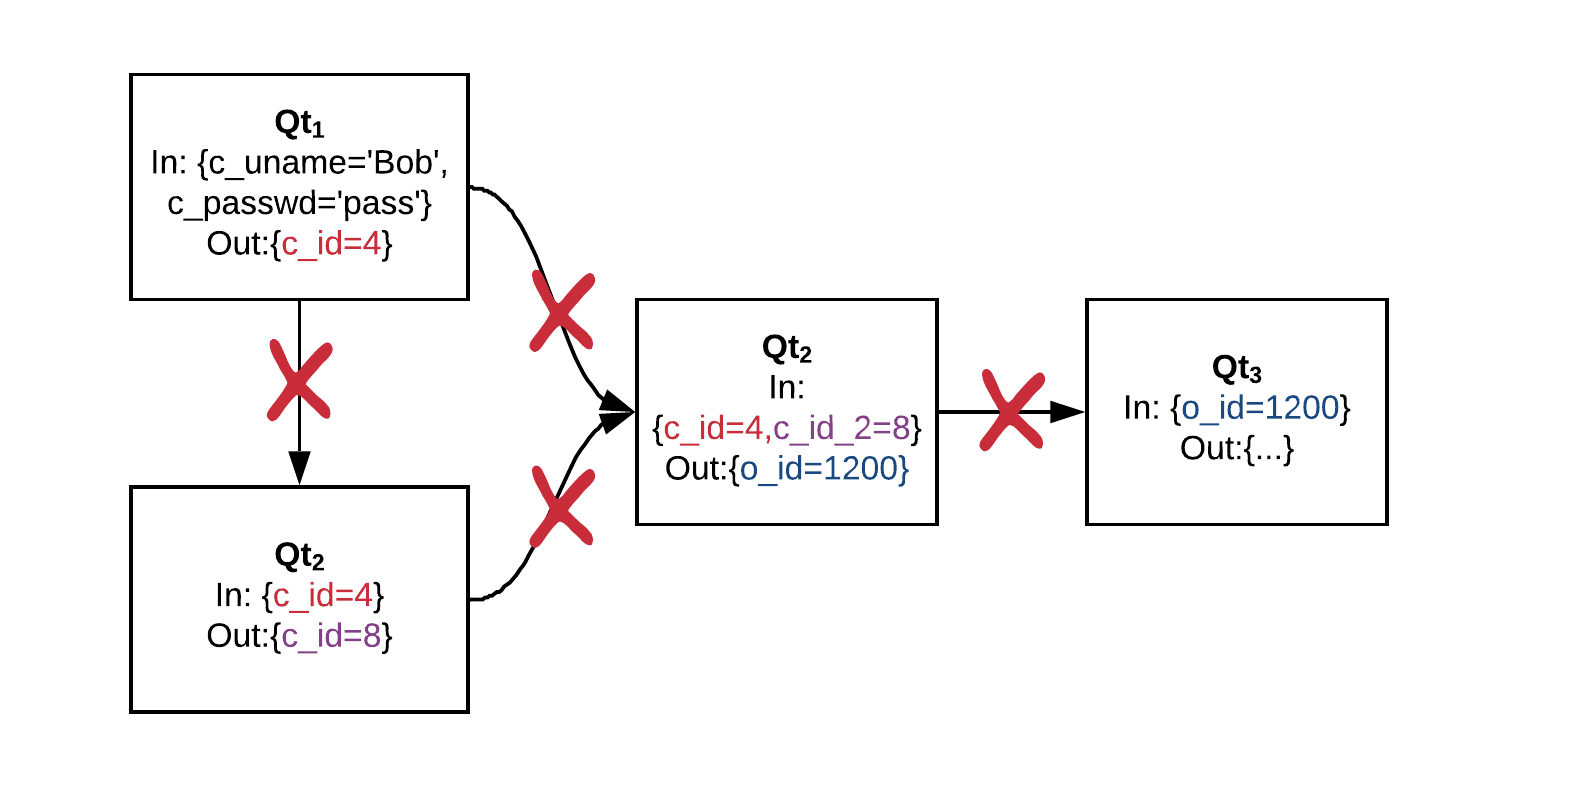
\includegraphics[scale=0.22]{apollo_cpr}
    \end{figure}
\end{frame}

\begin{frame}[fragile]{Always Defined Queries}
    An \alert{always defined query} (ADQ) is an FDQ where all of its prior queries (recursively) are also FDQs.\\
\medskip
    \visible<2->{
       In other words, its dependencies are \alert{always satisfied}, and the query can be executed and cached at any time! 
    }
\end{frame}

\begin{frame}[fragile]{ADQ Reload}
Reload an ADQ if:
\begin{itemize}
    \visible<2->{
    \item{The ADQ is \alert{not} already cached}
    }
    \visible<3->{
    \item{The ADQ is considered \alert{valuable}: \\
$P(\mathit{Qt})\cdot C(\mathit{Qt}) \geq \alpha$
    }
    }
\end{itemize}
\end{frame}

\section{Apollo}

\begin{frame}[fragile]{Apollo Overview}
    \begin{figure}
        \hspace*{-1cm}
        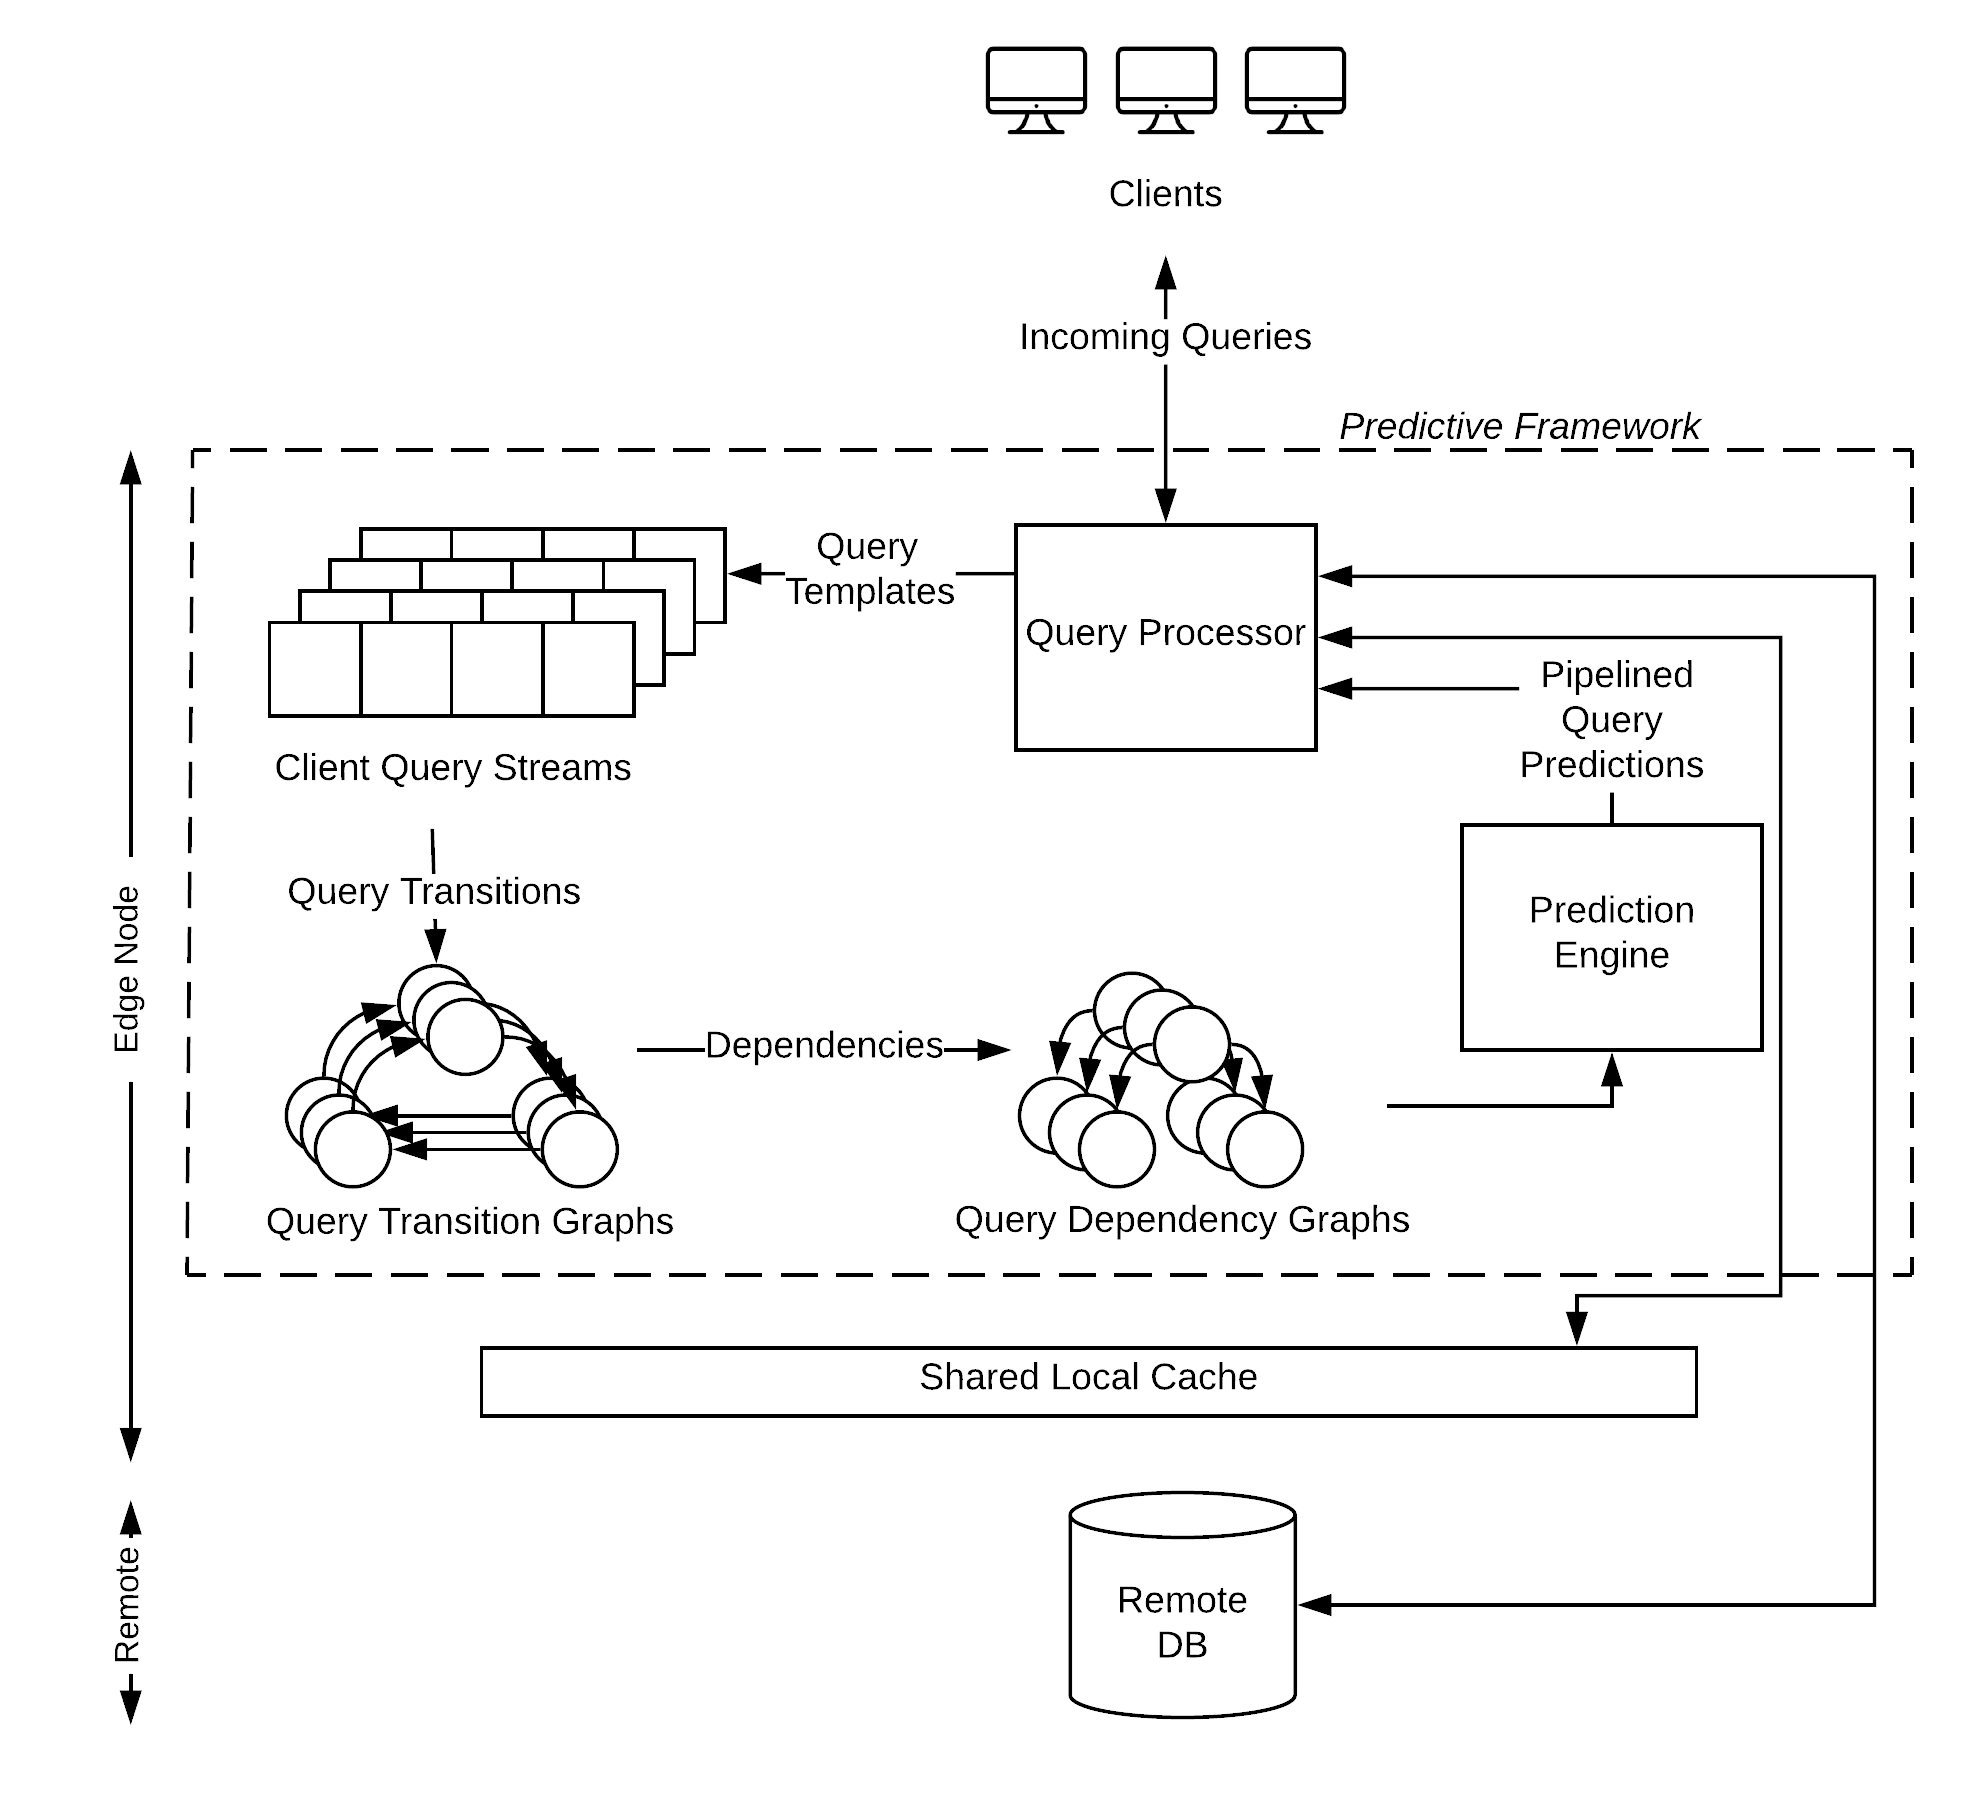
\includegraphics[scale=0.13]{apollo_overview}
    \end{figure}
\end{frame}

\begin{frame}[fragile]{Apollo Overview}
    \begin{figure}
        \hspace*{-1cm}
        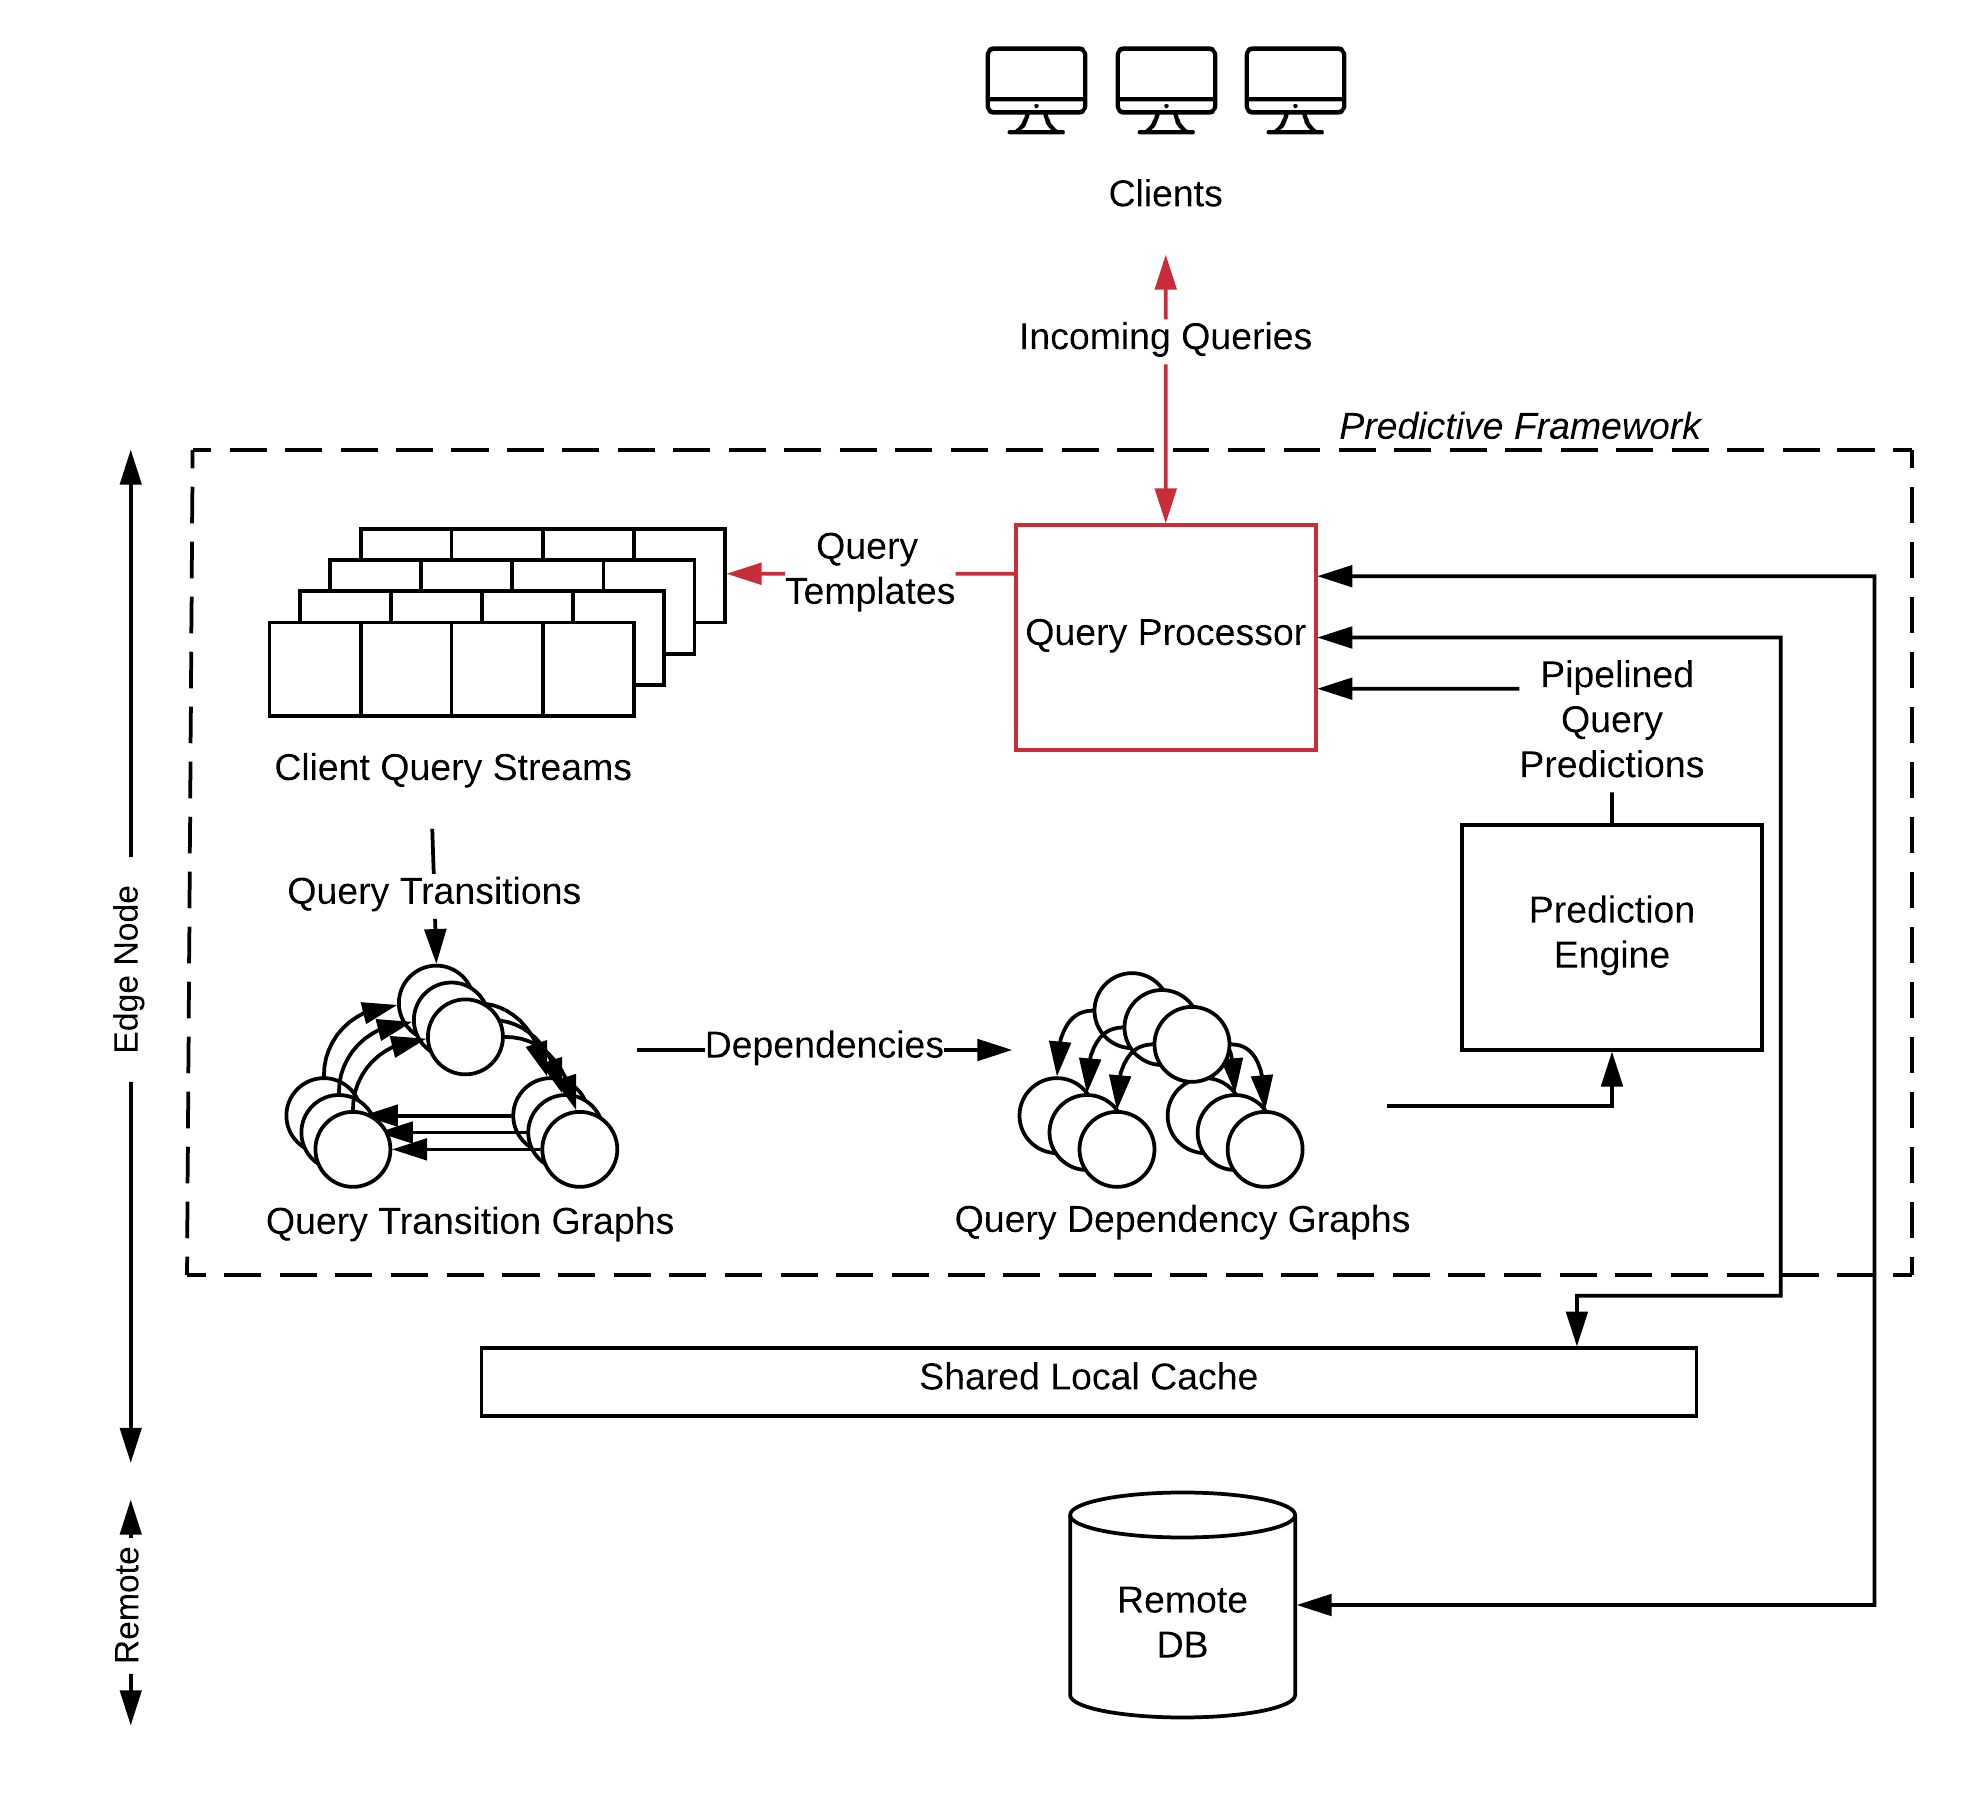
\includegraphics[scale=0.13]{apollo_overview_2}
    \end{figure}
\end{frame}

\begin{frame}[fragile]{Apollo Overview}
    \begin{figure}
        \hspace*{-1cm}
        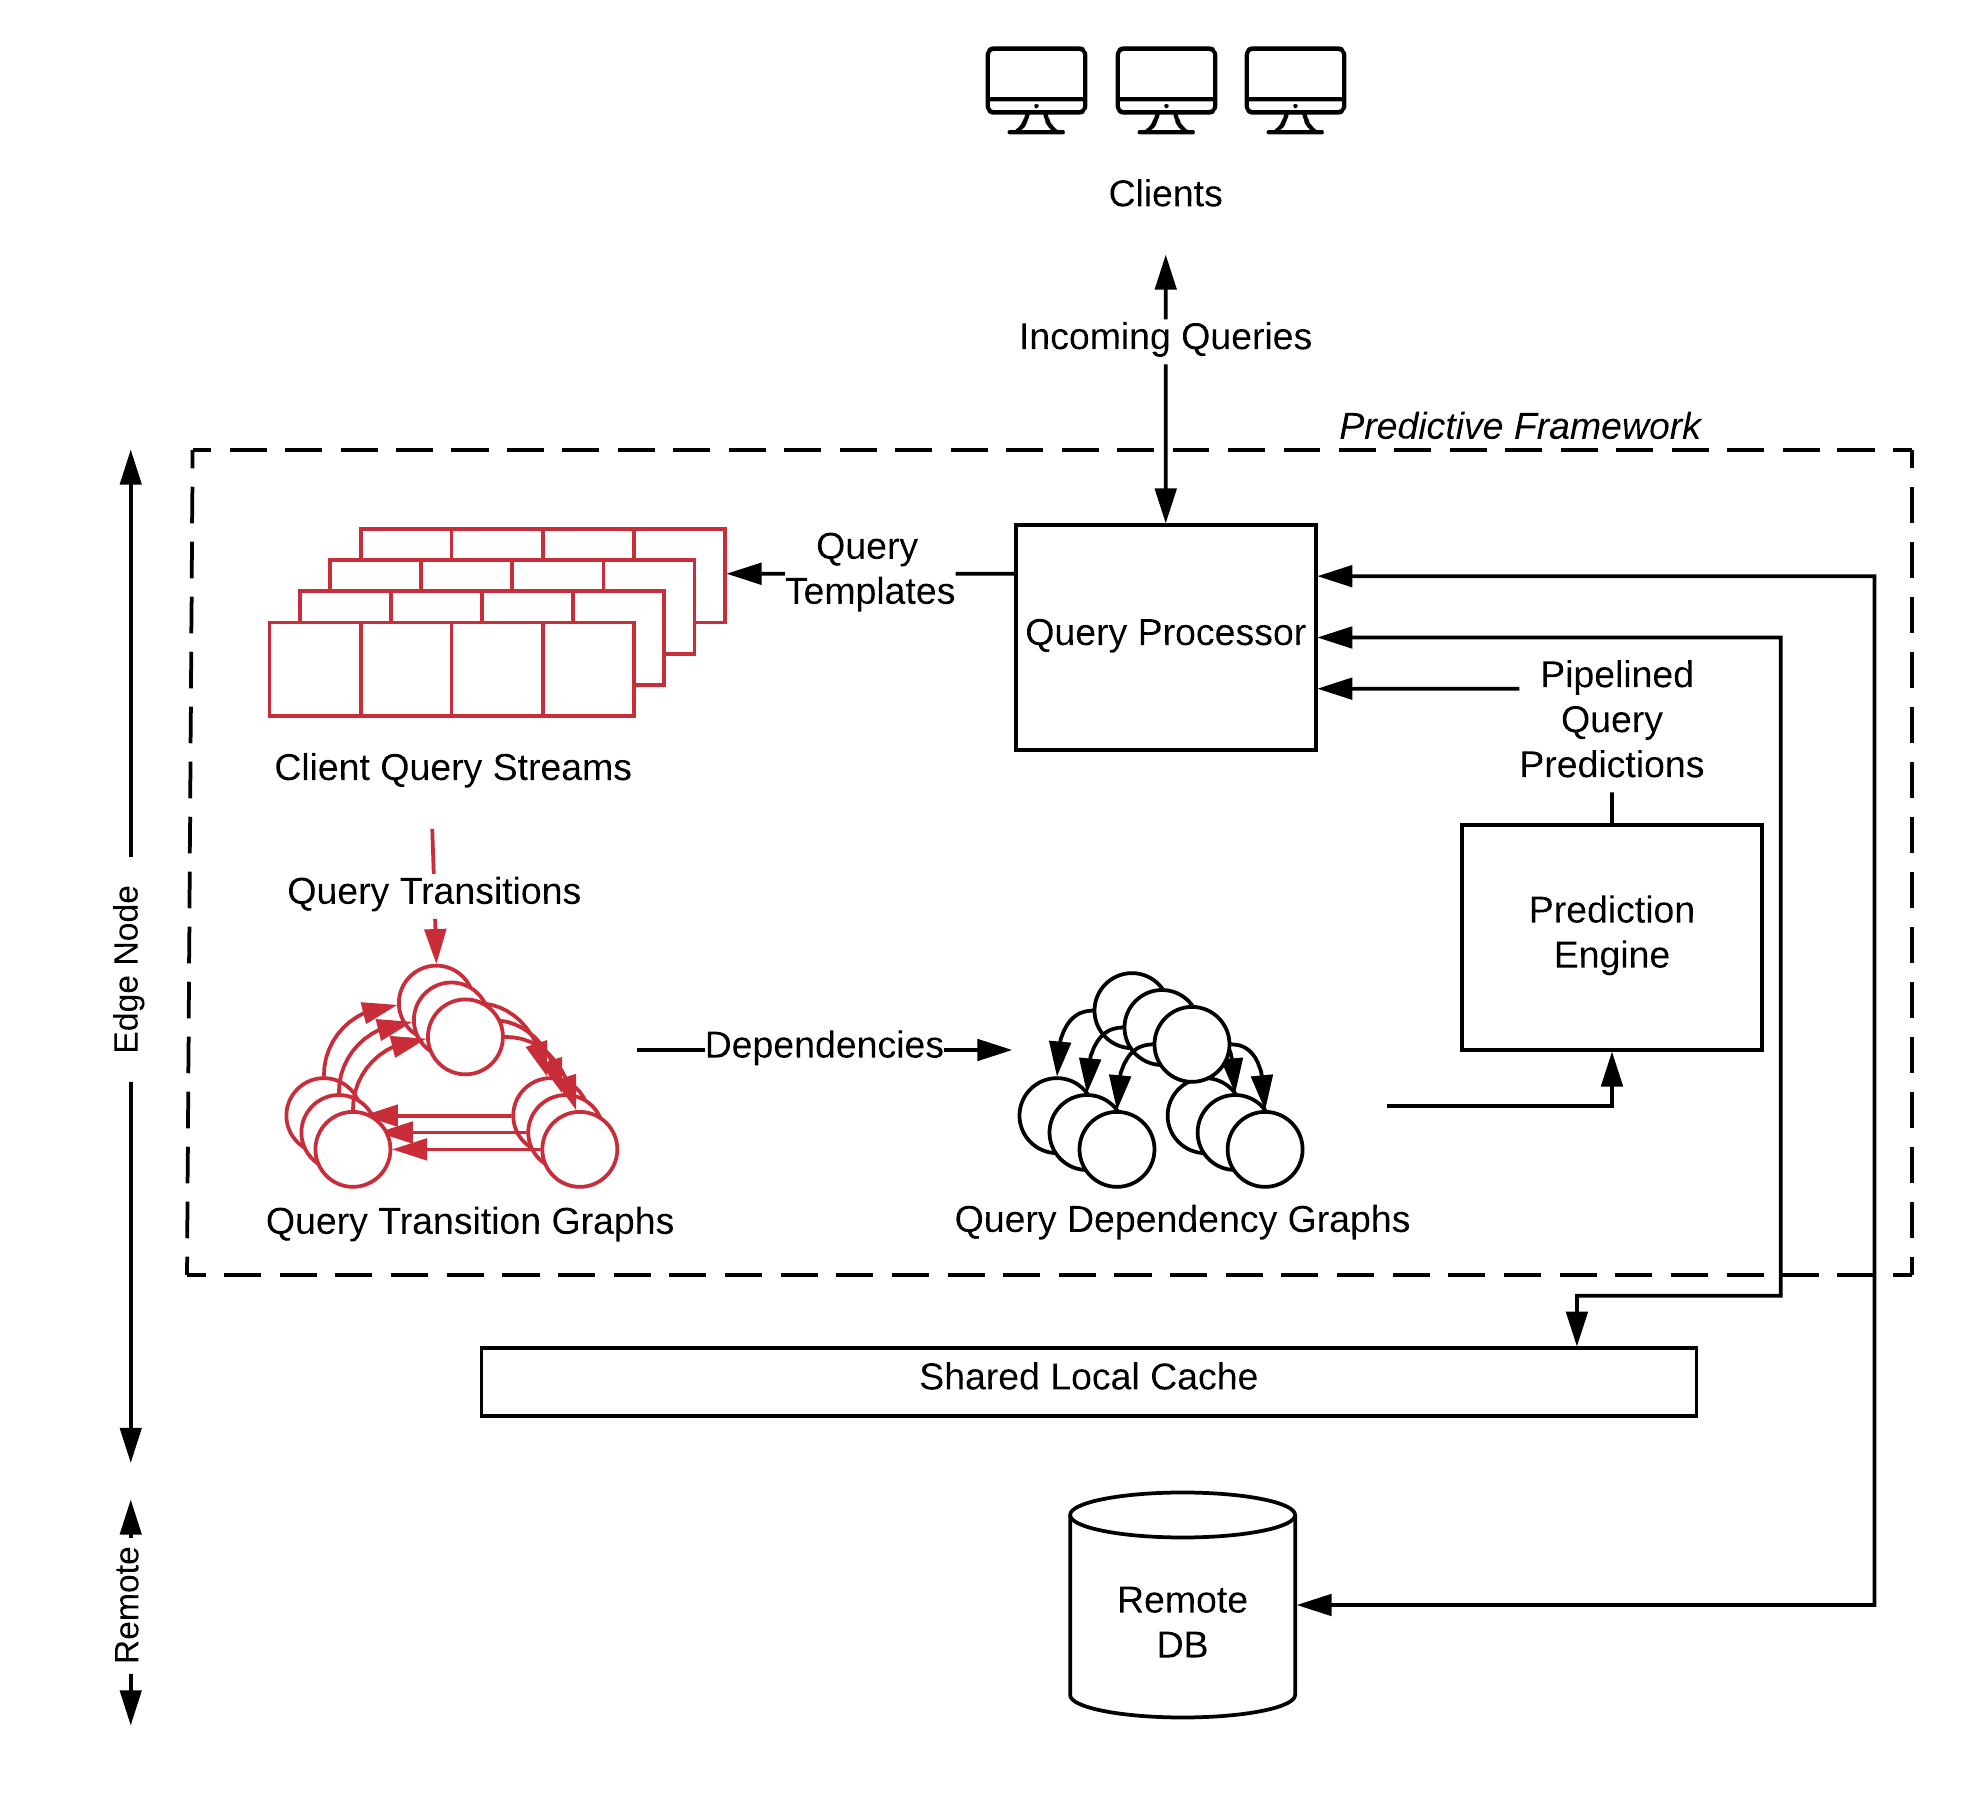
\includegraphics[scale=0.13]{apollo_overview_3}
    \end{figure}
\end{frame}

\begin{frame}[fragile]{Apollo Overview}
    \begin{figure}
        \hspace*{-1cm}
        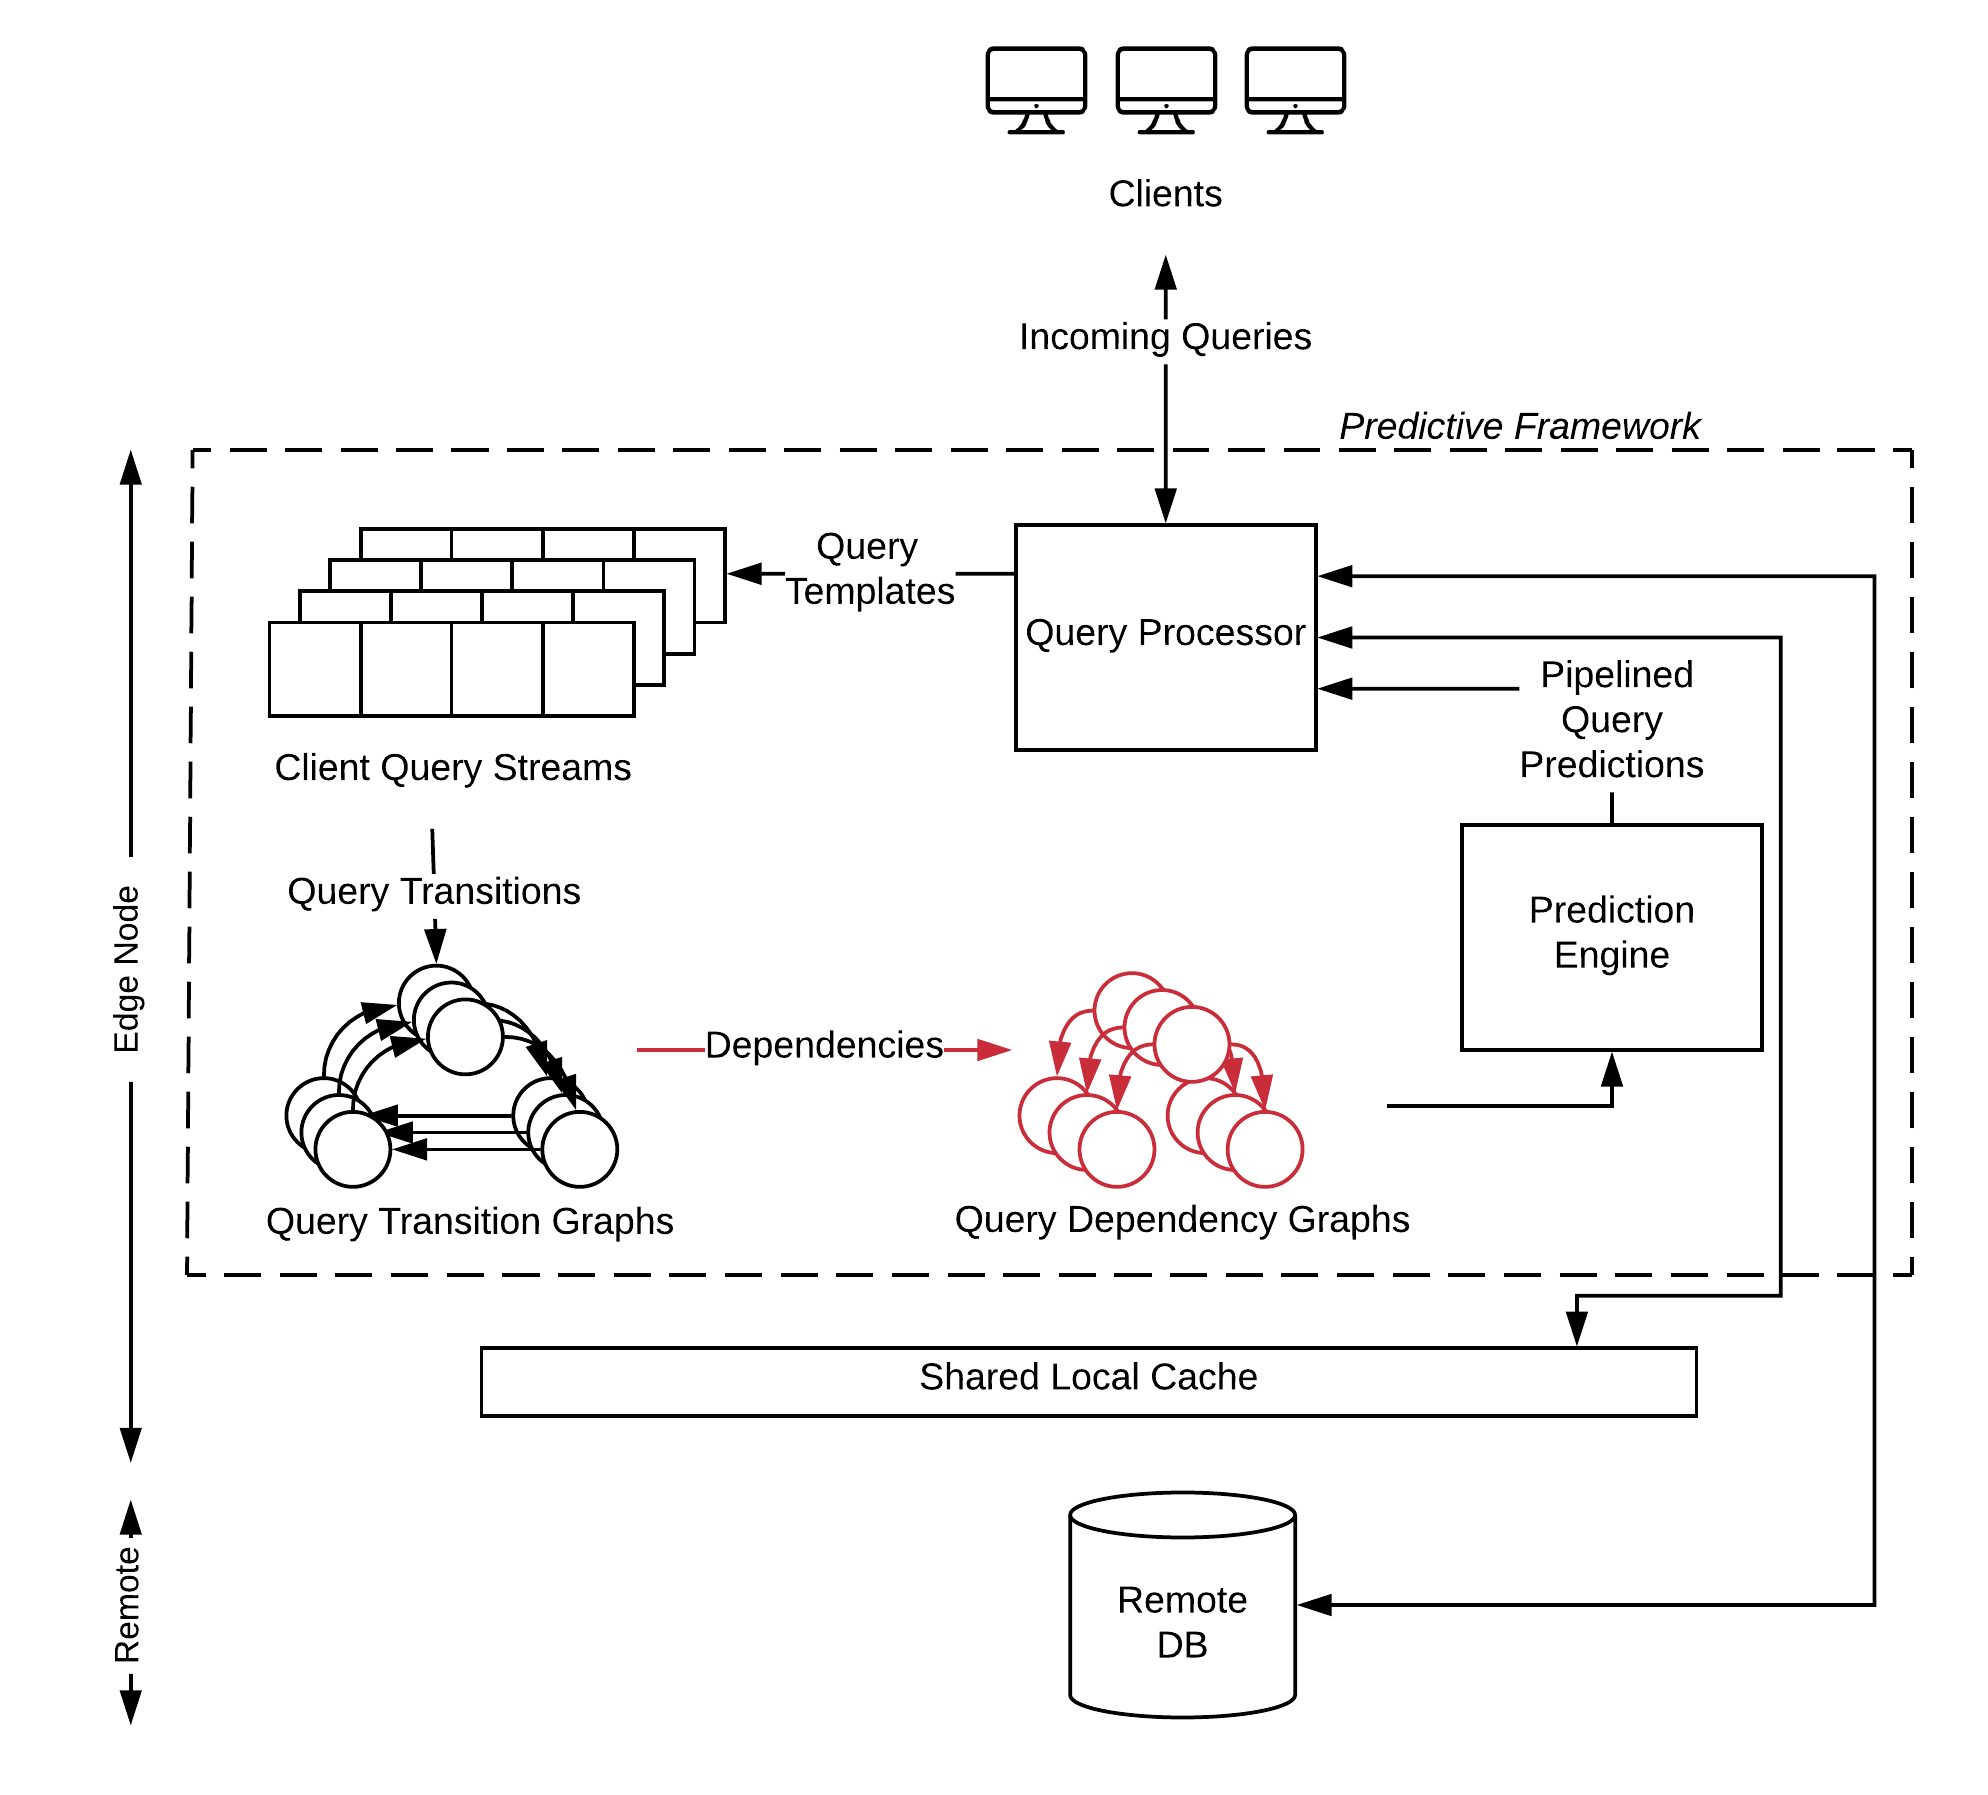
\includegraphics[scale=0.13]{apollo_overview_4}
    \end{figure}
\end{frame}

\begin{frame}[fragile]{Apollo Overview}
    \begin{figure}
        \hspace*{-1cm}
        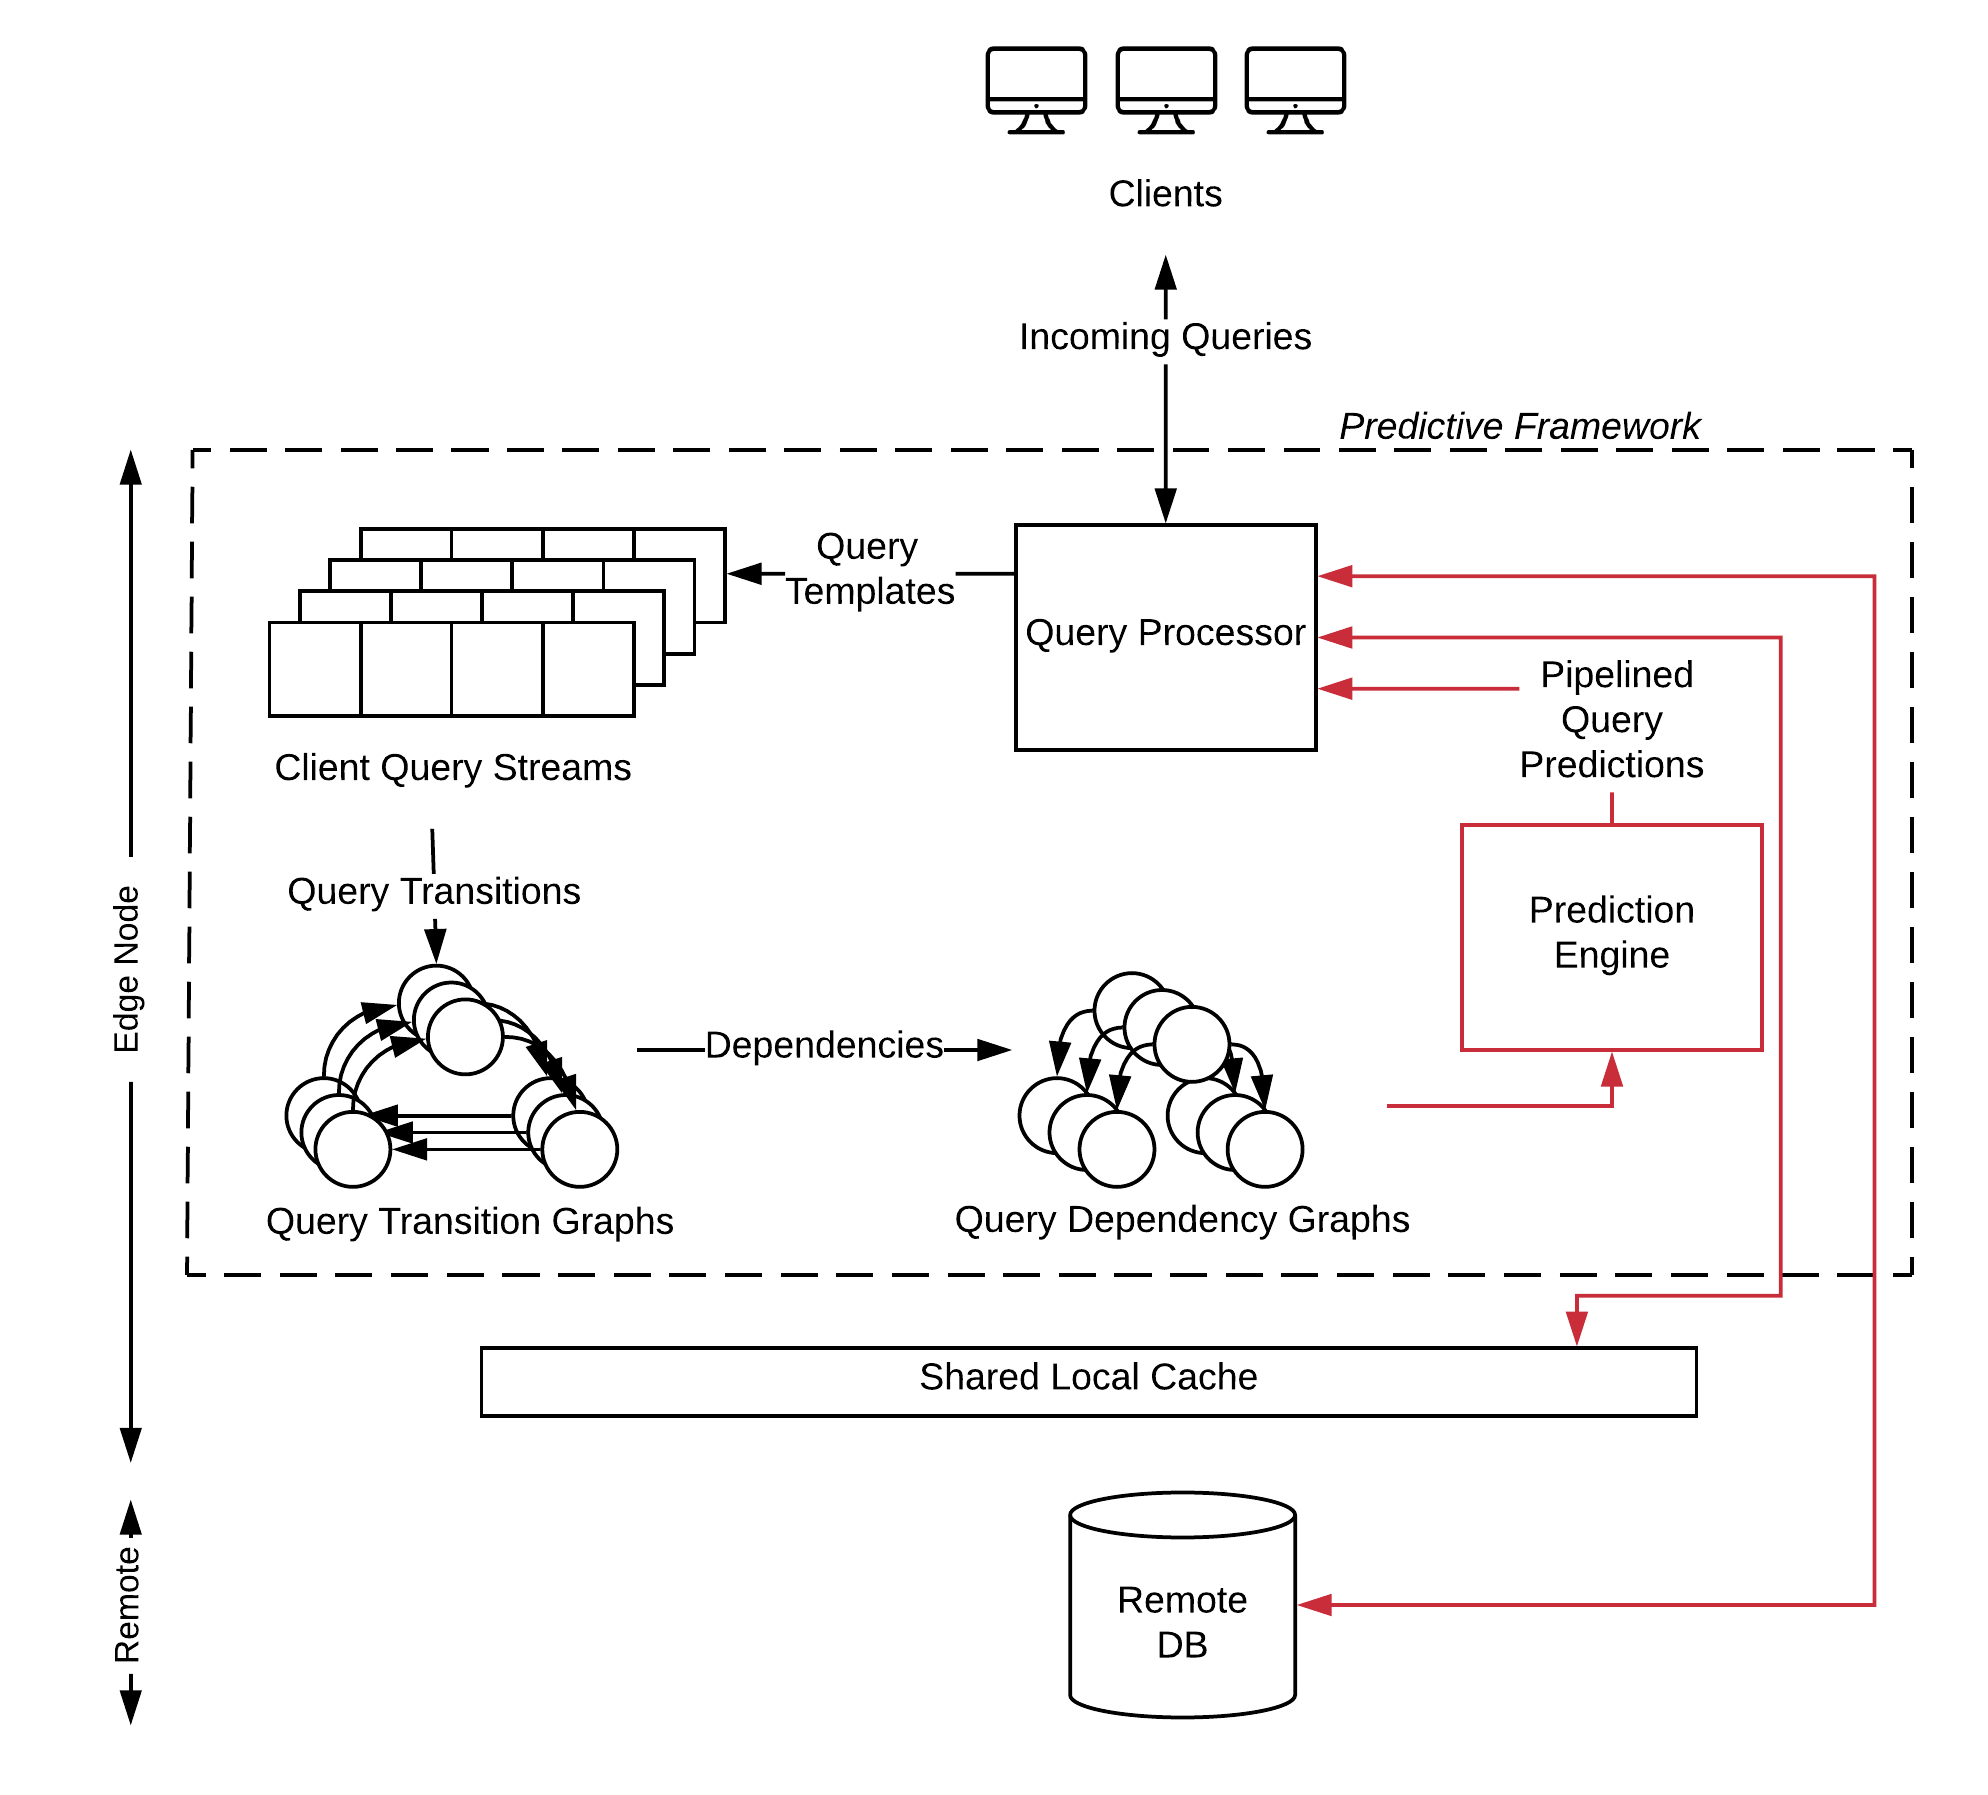
\includegraphics[scale=0.13]{apollo_overview_5}
    \end{figure}
\end{frame}

\begin{frame}[fragile]{Apollo Overview}
    \begin{figure}
        \hspace*{-1cm}
        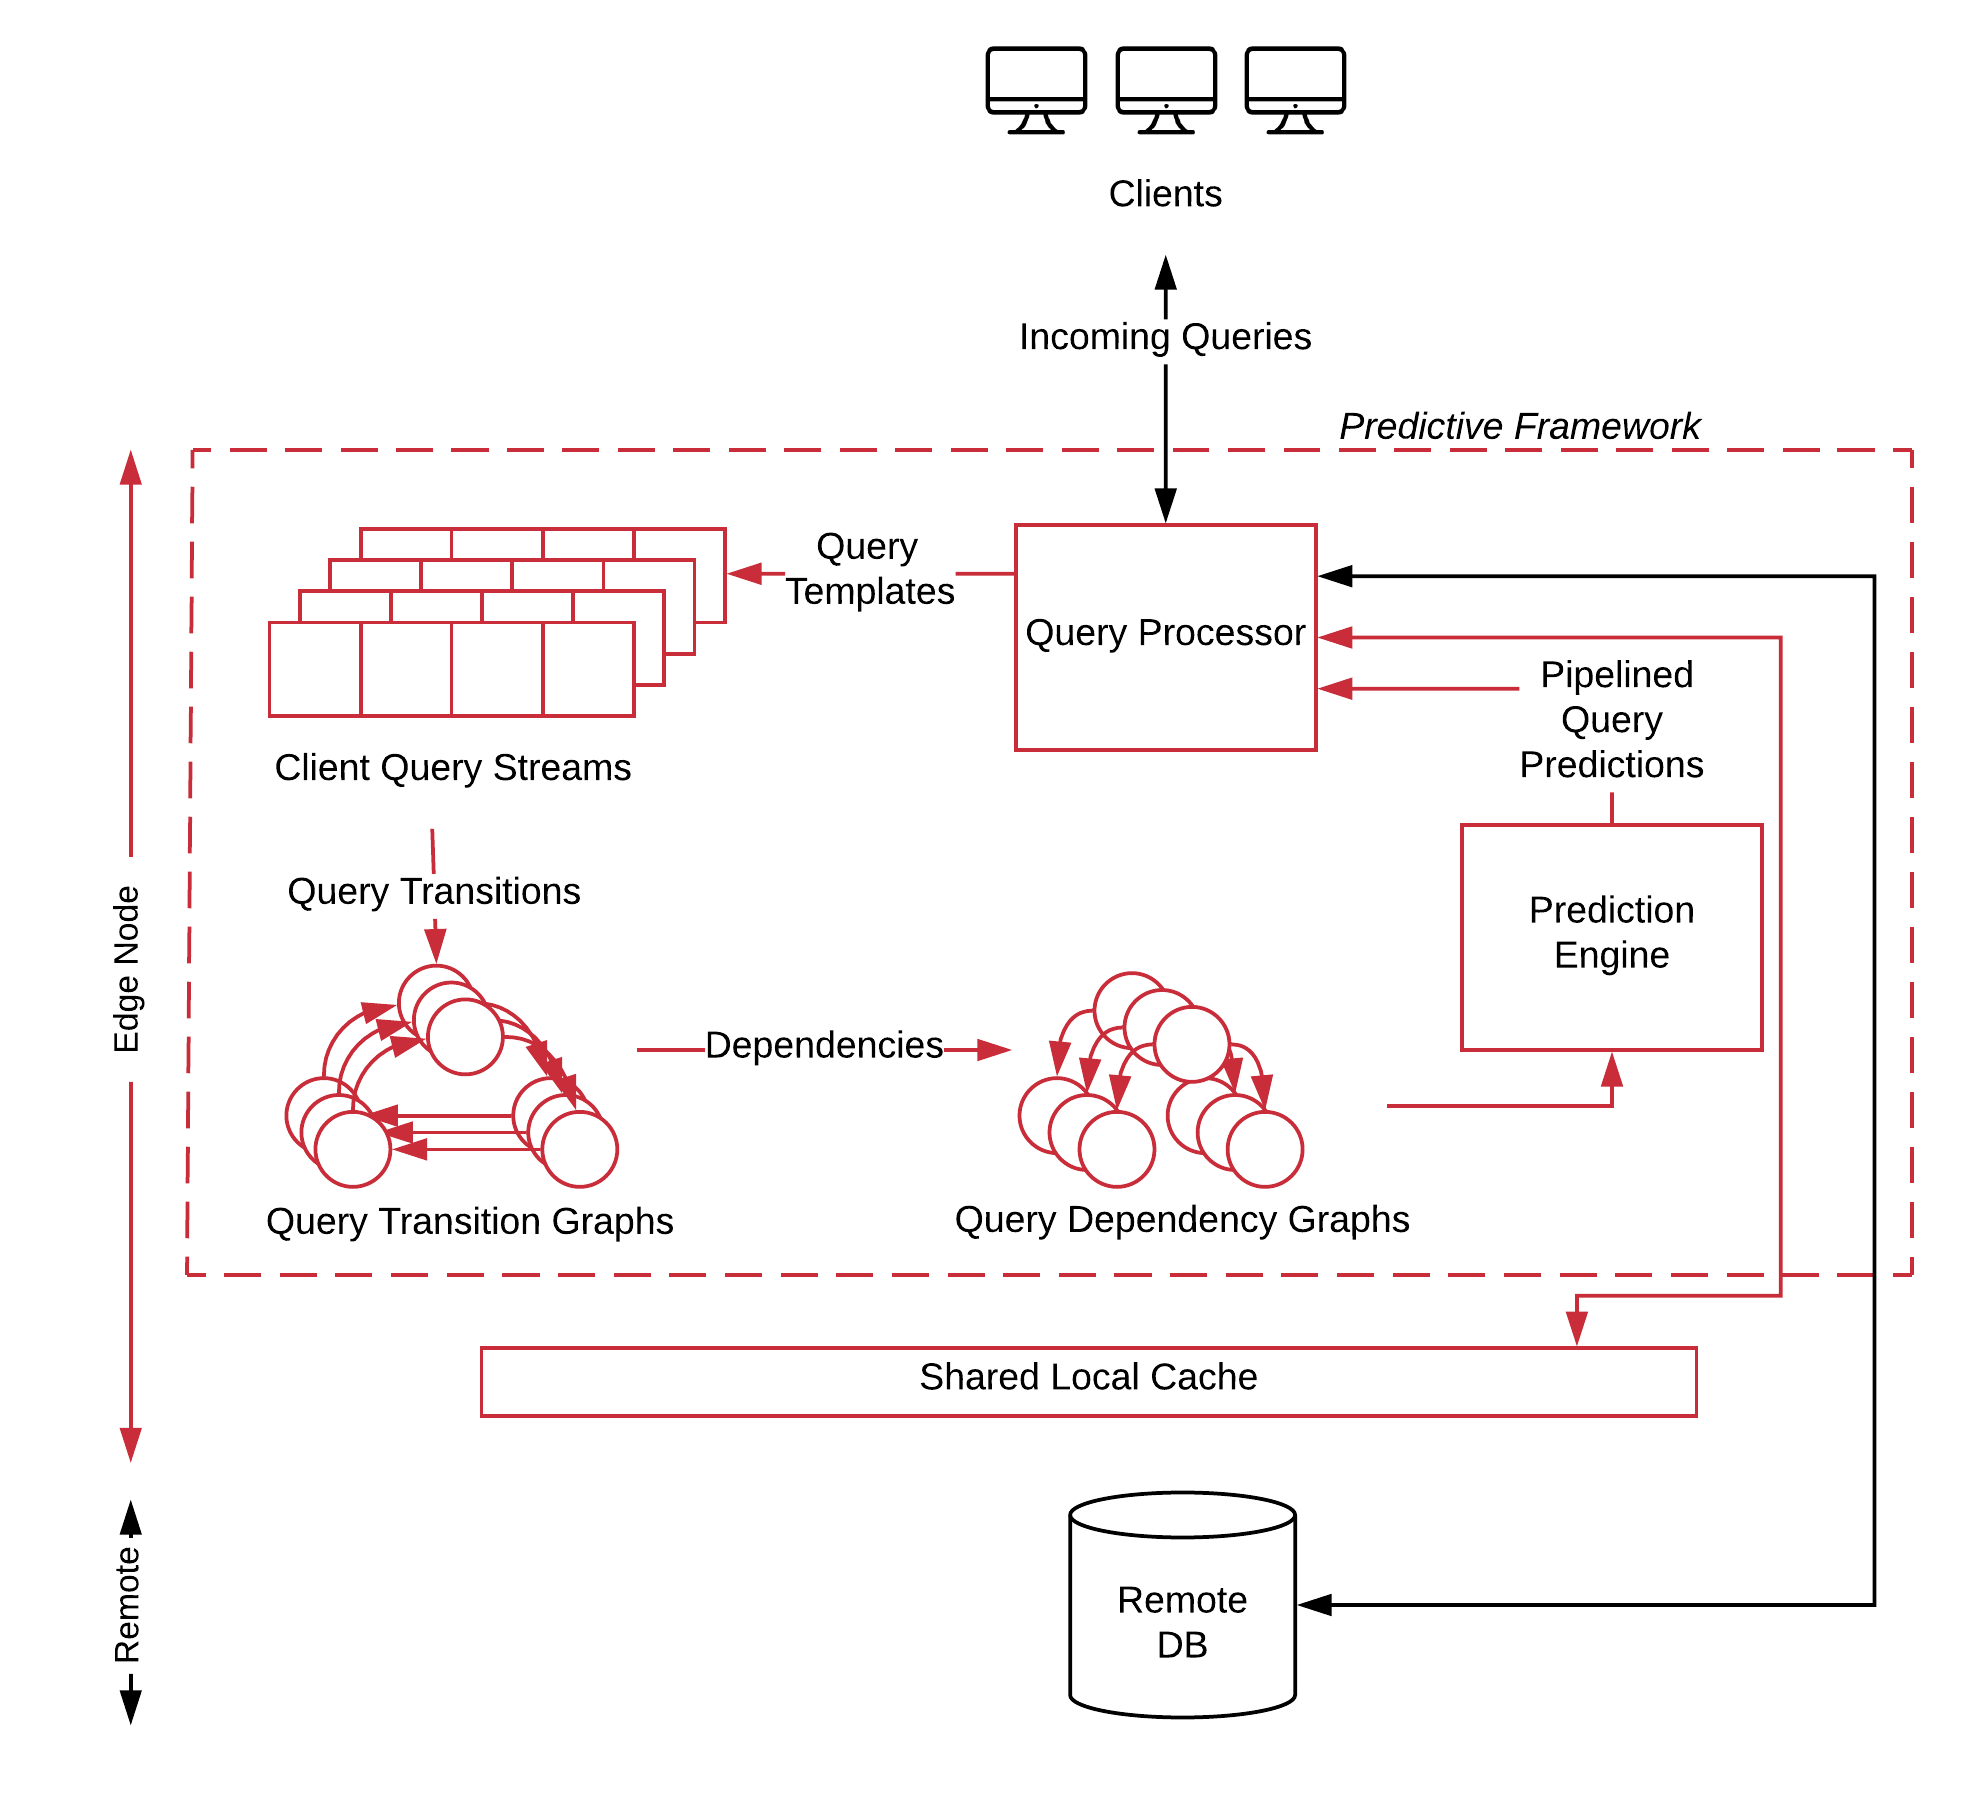
\includegraphics[scale=0.13]{apollo_overview_6}
    \end{figure}
\end{frame}

\begin{frame}[fragile]{Apollo Overview}
    \begin{figure}
        \hspace*{-1cm}
        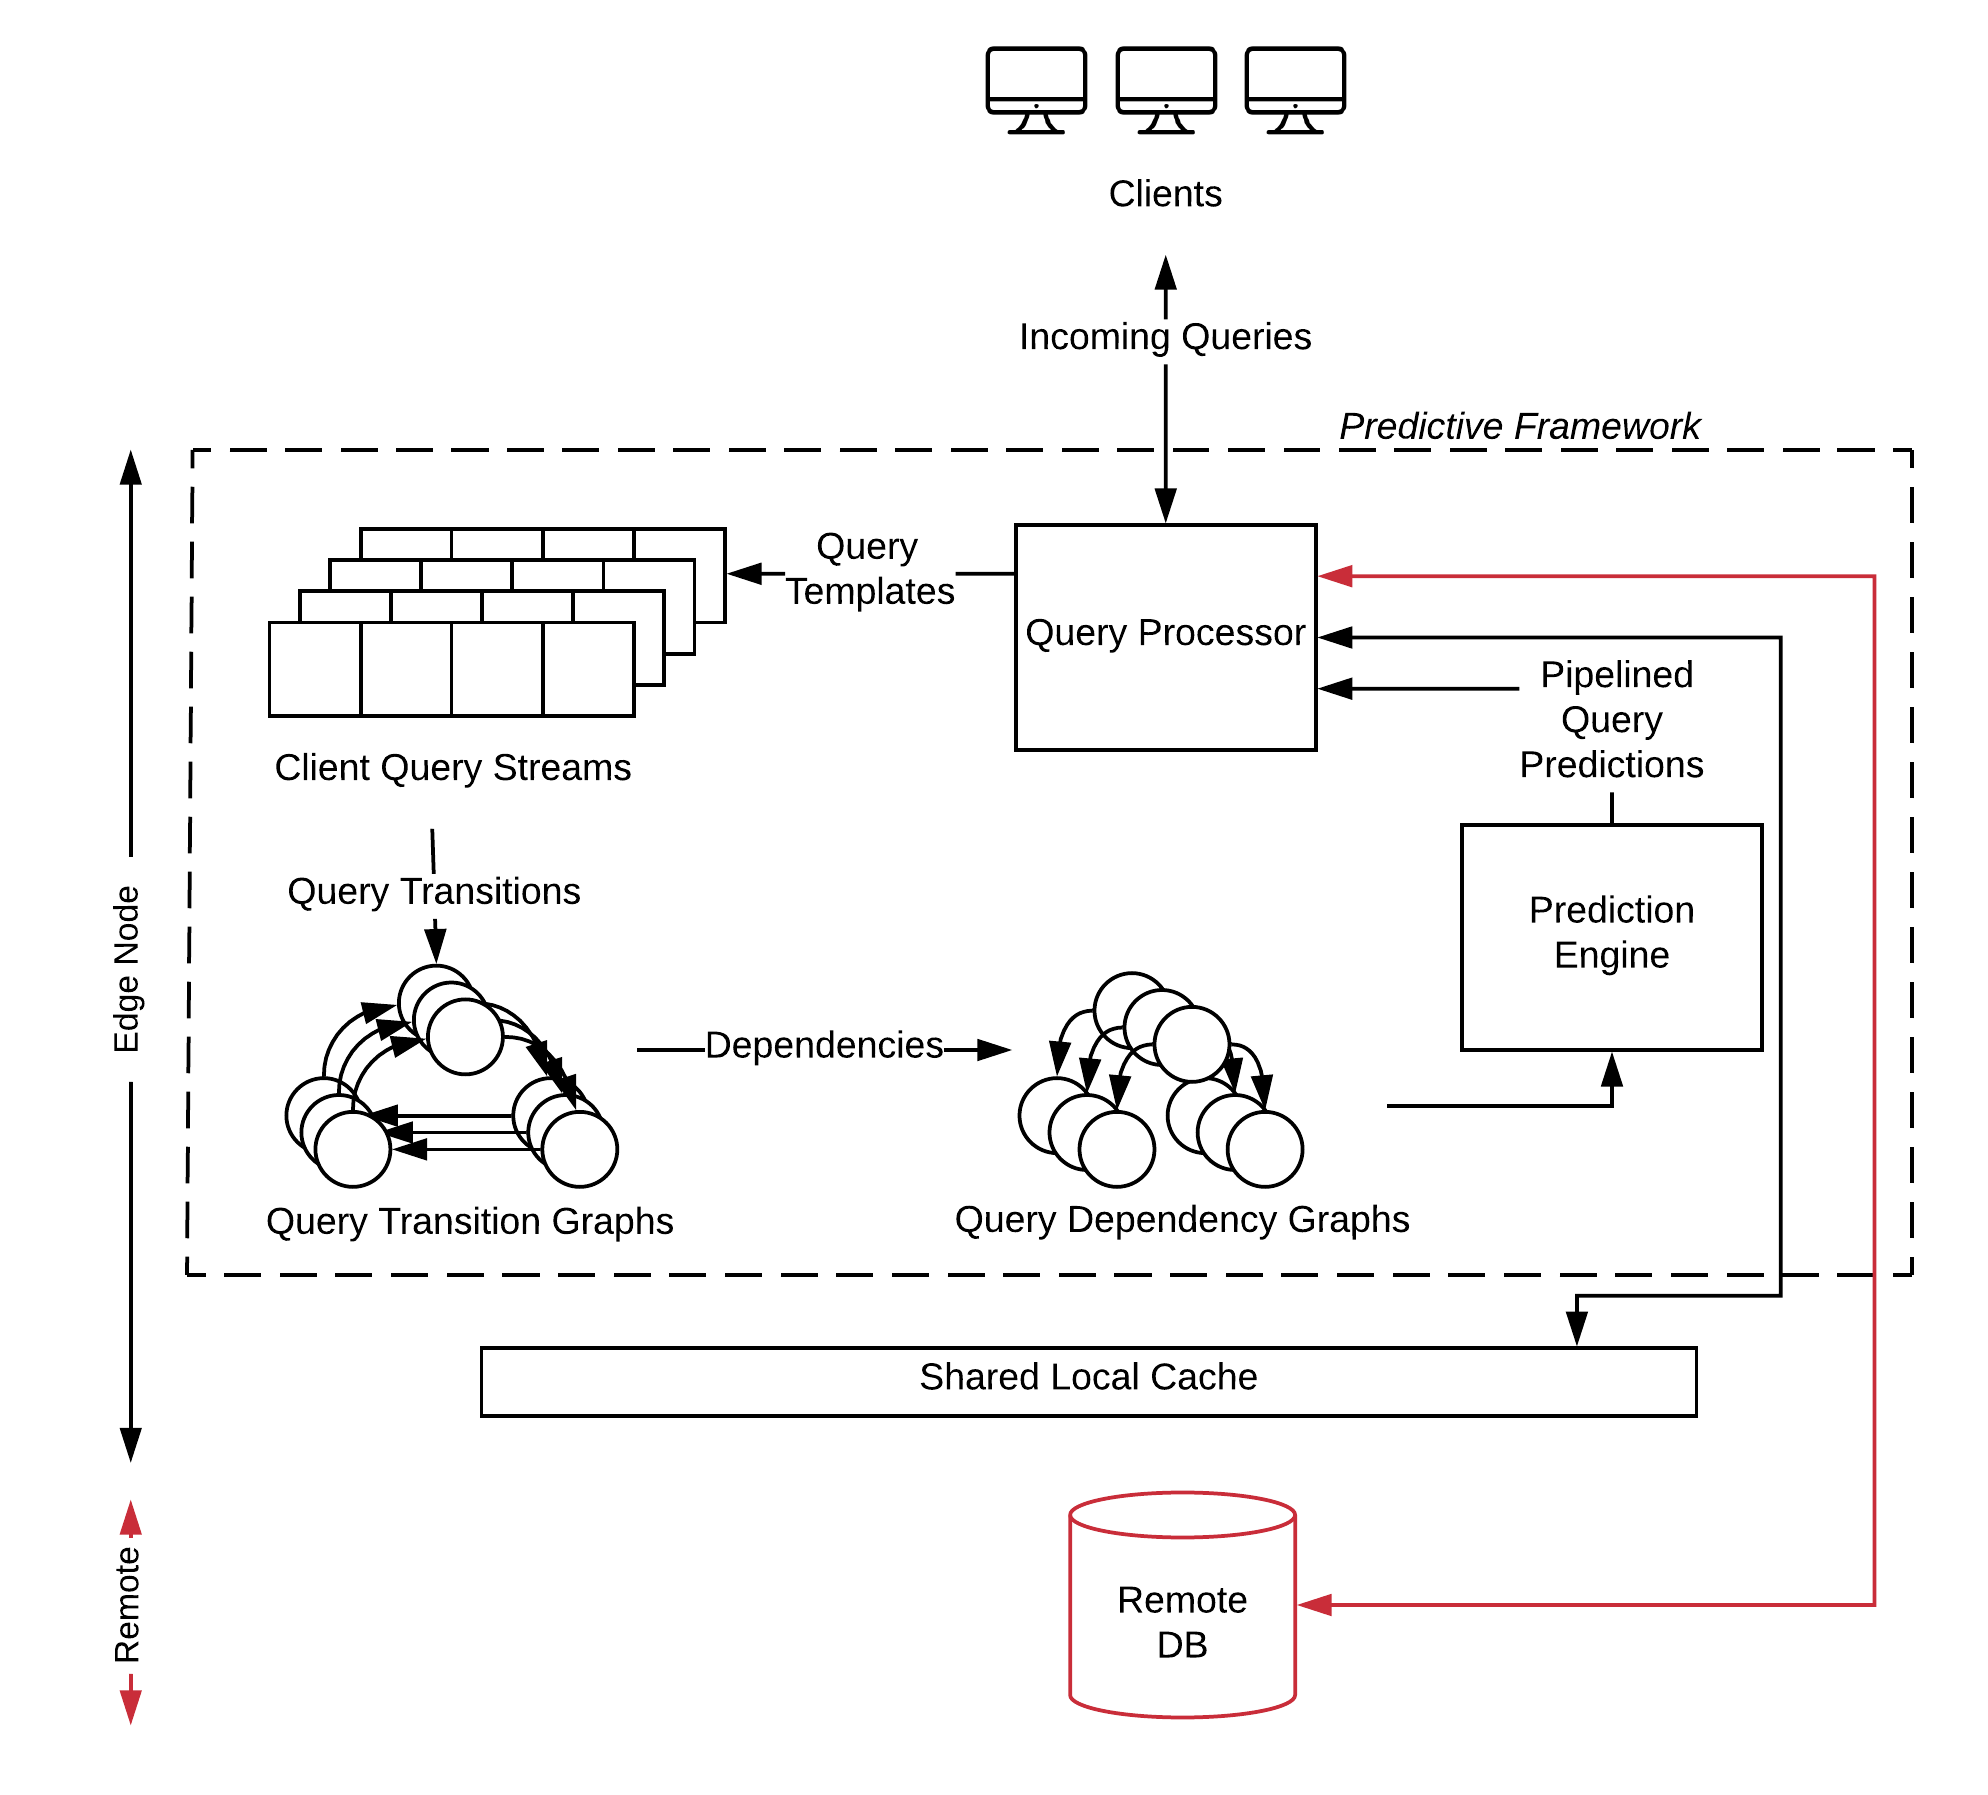
\includegraphics[scale=0.13]{apollo_overview_7}
    \end{figure}
\end{frame}

\begin{frame}[fragile]{Insert Oz Map}
Insert Oz Map
\end{frame}

\begin{frame}[fragile]{Apollo Architecture}
    \begin{figure}
        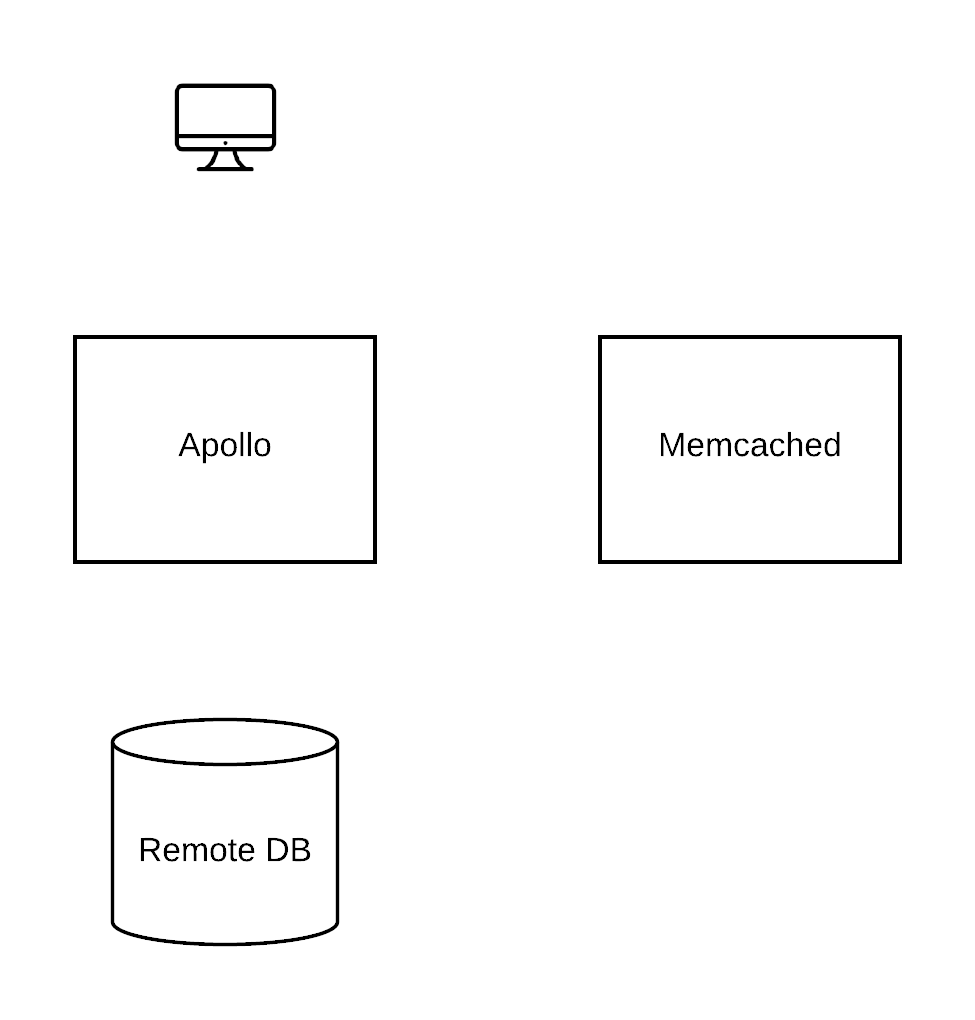
\includegraphics[scale=0.17]{apollo_arch_diagram}
    \end{figure}
\end{frame}

\begin{frame}[fragile]{Apollo Architecture}
    \begin{figure}
        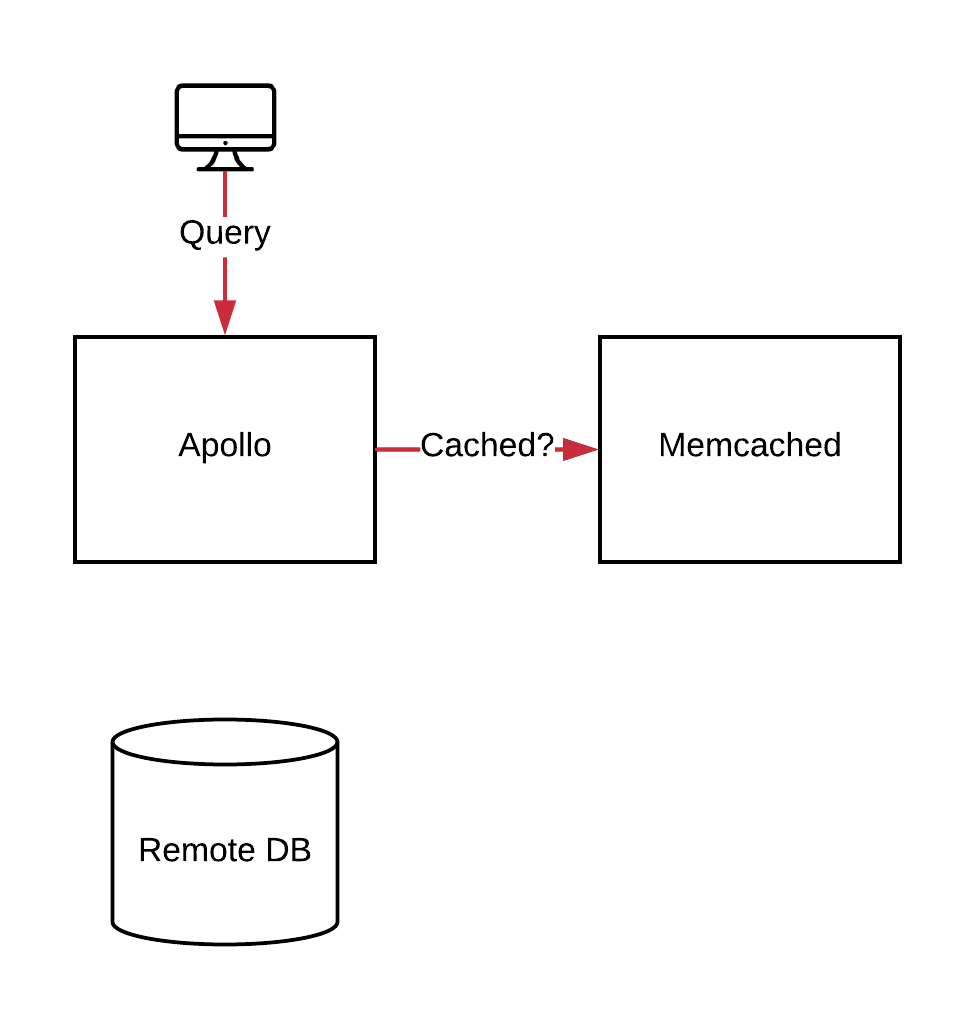
\includegraphics[scale=0.17]{apollo_arch_diagram_2}
    \end{figure}
\end{frame}

\begin{frame}[fragile]{Apollo Architecture}
    \begin{figure}
        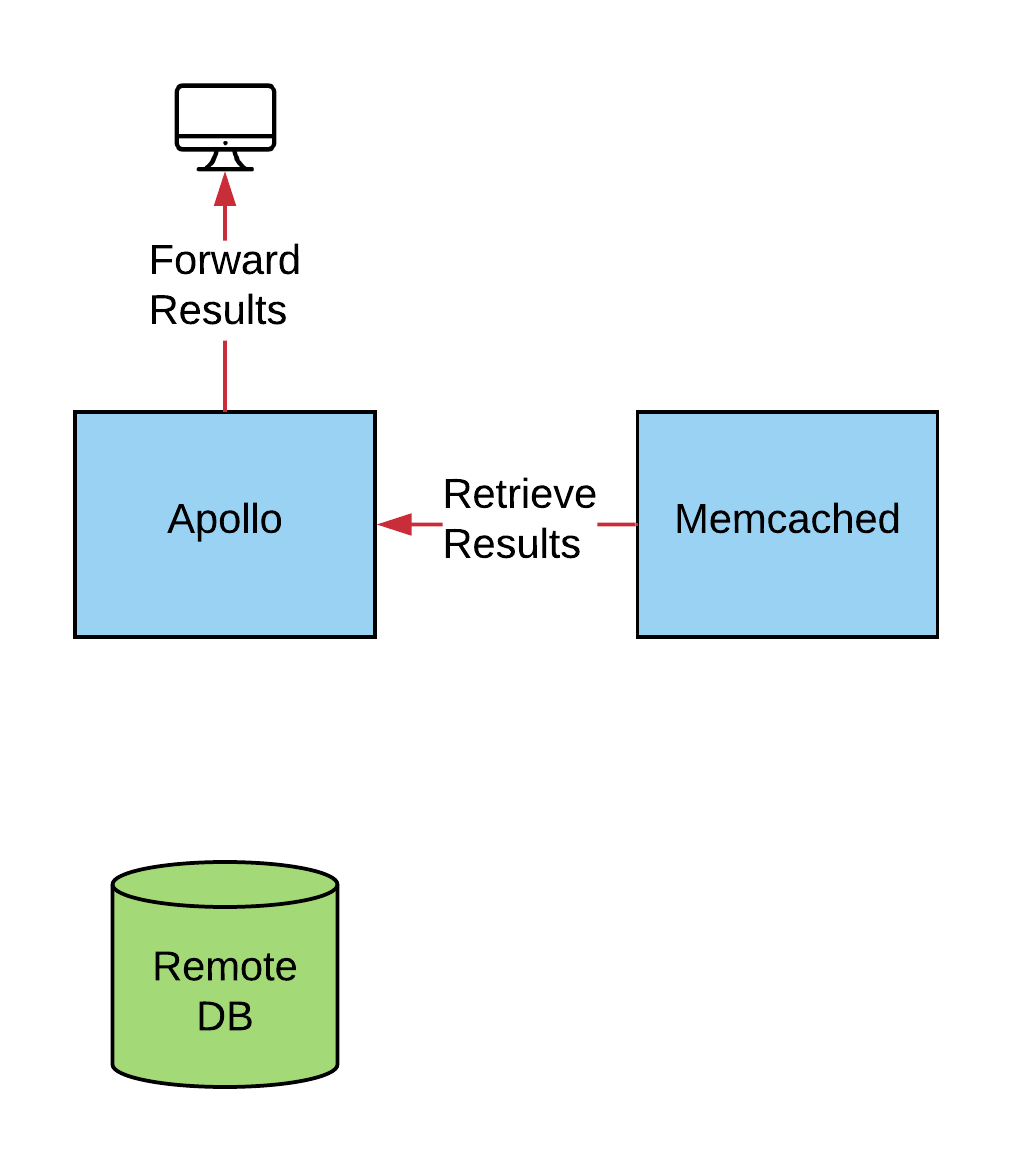
\includegraphics[scale=0.17]{apollo_arch_diagram_3}
    \end{figure}
\end{frame}

\begin{frame}[fragile]{Apollo Architecture}
    \begin{figure}
        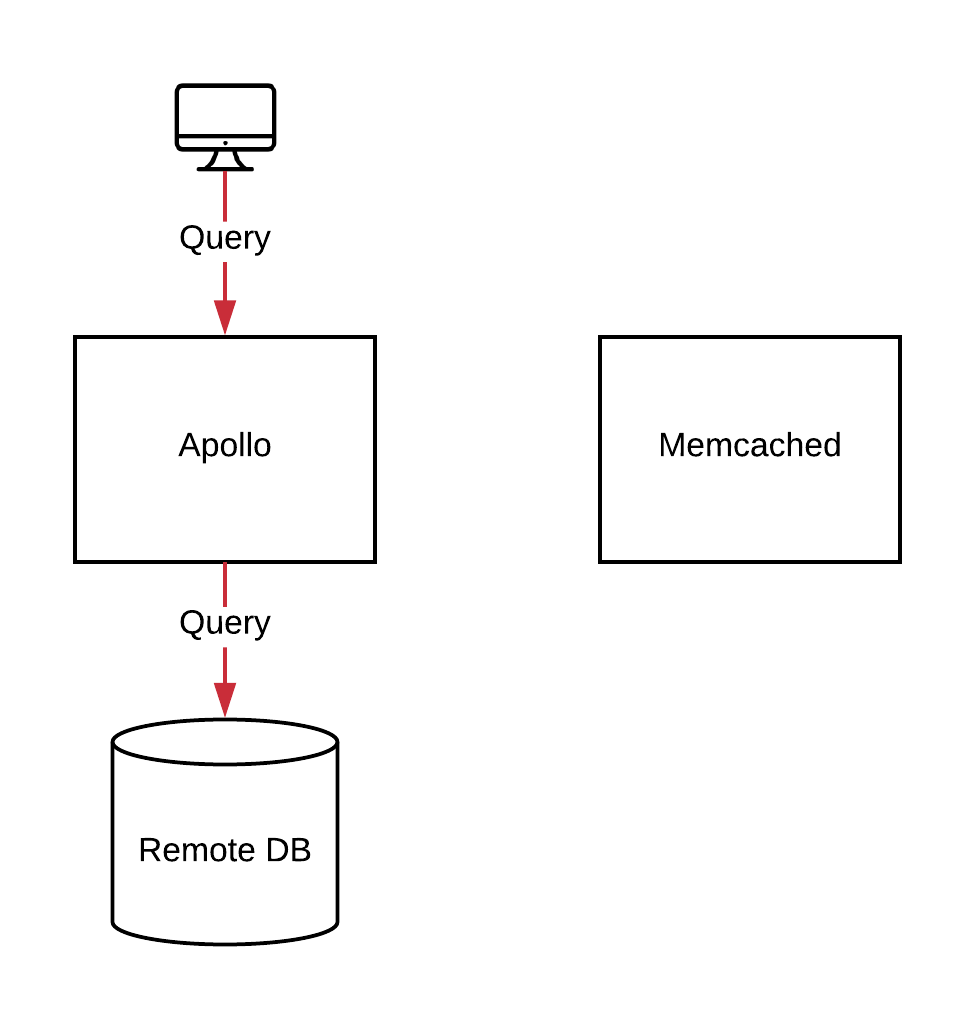
\includegraphics[scale=0.17]{apollo_arch_diagram_5}
    \end{figure}
\end{frame}

\begin{frame}[fragile]{Apollo Architecture}
    \begin{figure}
        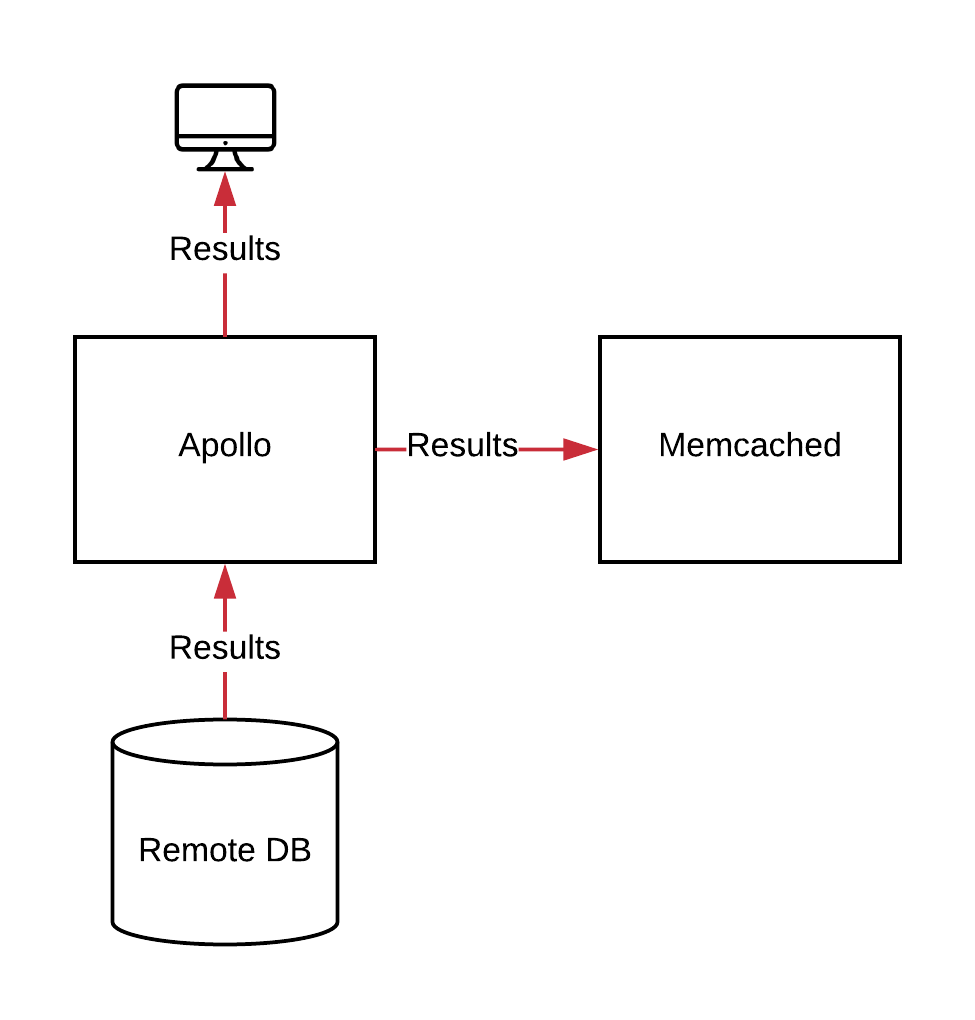
\includegraphics[scale=0.17]{apollo_arch_diagram_6}
    \end{figure}
\end{frame}

\begin{frame}[fragile]{Apollo Architecture}
    \begin{figure}
        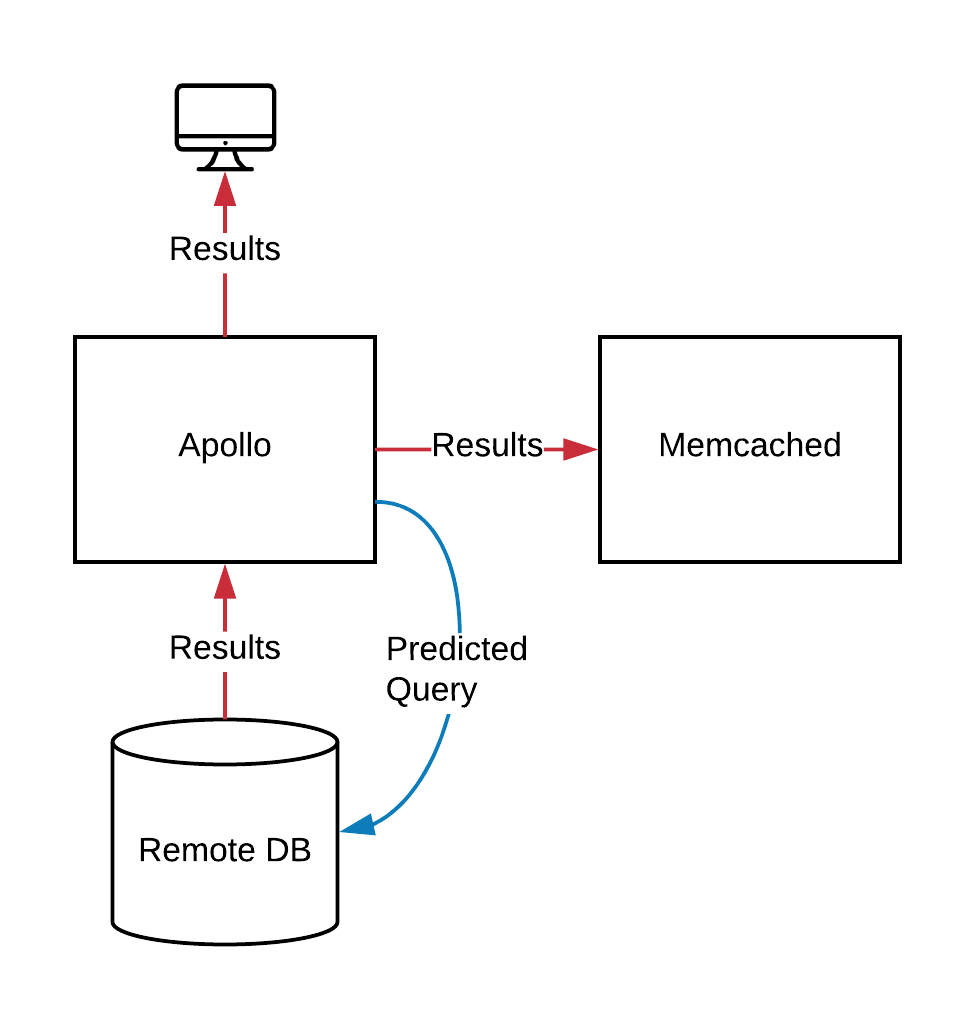
\includegraphics[scale=0.17]{apollo_arch_diagram_7}
    \end{figure}
\end{frame}

\begin{frame}[fragile]{Apollo Architecture}
    \begin{figure}
        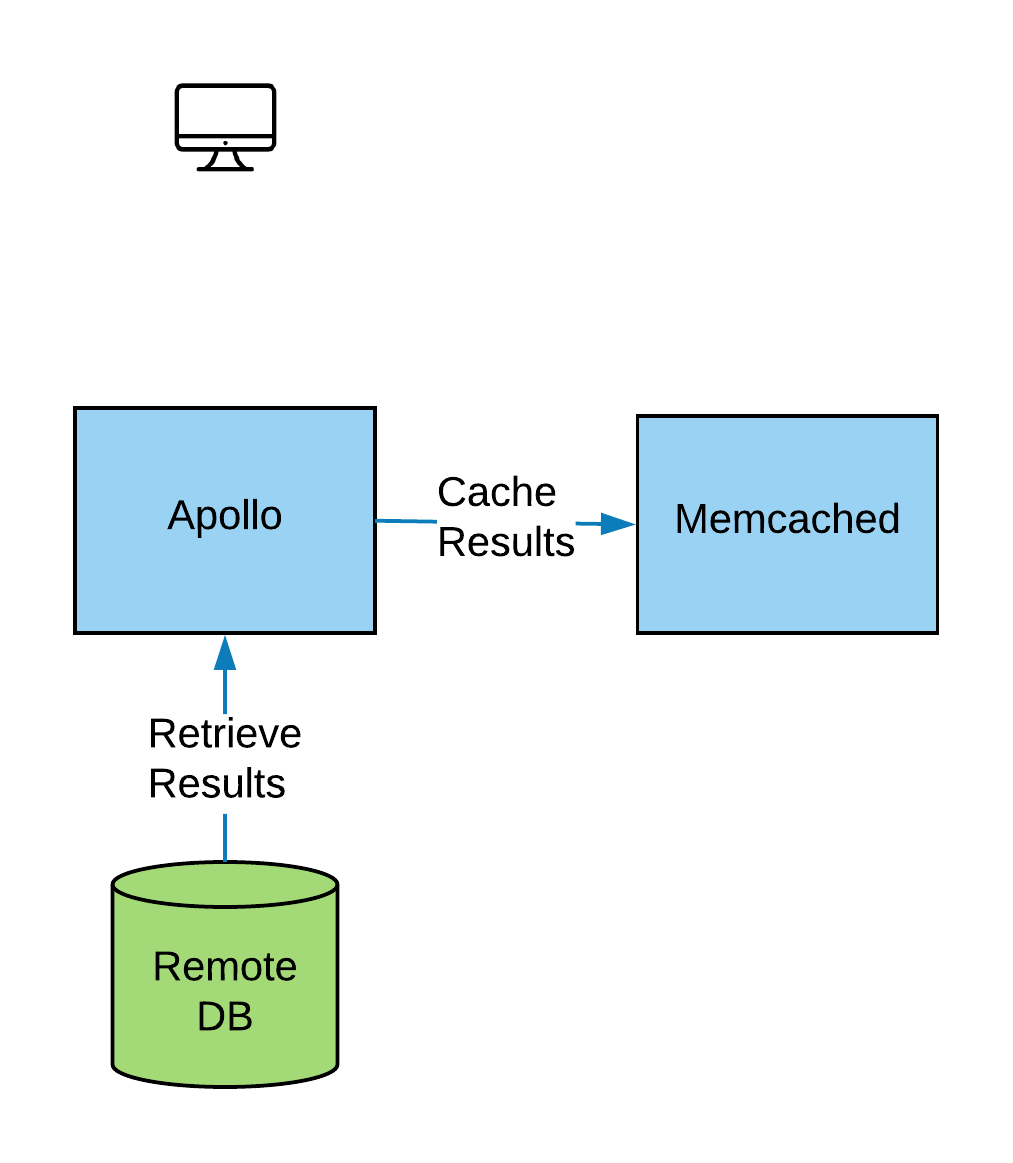
\includegraphics[scale=0.17]{apollo_arch_diagram_8}
    \end{figure}
\end{frame}

\begin{frame}[fragile]{Cache Matching}
Key query results by \alert{hash of query template}.
\begin{itemize}
    \item{Fast lookup for incoming queries}
    \item{Avoids \alert{query containment}, but cannot use portions of result sets shared by other queries}
\end{itemize}
\end{frame}

\begin{frame}[fragile]{Cache Invalidation}
Standard approaches to invalidate caches will not scale globally!\\
\medskip
\visible<2->{
Use \alert{client sessions} and Memcached's LRU to invalidate and implicitly evict
}
\end{frame}

\begin{frame}[fragile]{Client Sessions}
Clients are guaranteed to see state at least as recent as what they last read/wrote.
\end{frame}

\begin{frame}[fragile]{Client Sessions}
    \begin{figure}
        \includegraphics[scale=0.17]{apollo_client_sessions}
    \end{figure}
\end{frame}

\begin{frame}[fragile]{Client Sessions}
    \begin{figure}
        \includegraphics[scale=0.17]{apollo_client_sessions_2}
    \end{figure}
\end{frame}

\begin{frame}[fragile]{Client Sessions}
    \begin{figure}
        \includegraphics[scale=0.17]{apollo_client_sessions_3}
    \end{figure}
\end{frame}

\begin{frame}[fragile]{Client Sessions}
    \begin{figure}
        \includegraphics[scale=0.17]{apollo_client_sessions_4}
    \end{figure}
\end{frame}

\begin{frame}[fragile]{Client Sessions}
    \begin{figure}
        \includegraphics[scale=0.17]{apollo_client_sessions_6}
    \end{figure}
\end{frame}

\begin{frame}[fragile]{Client Sessions}
    \begin{figure}
        \includegraphics[scale=0.17]{apollo_client_sessions_7}
    \end{figure}
\end{frame}

\begin{frame}[fragile]{Client Sessions}
    \begin{figure}
        \includegraphics[scale=0.17]{apollo_client_sessions_8}
    \end{figure}
\end{frame}

\begin{frame}[fragile]{Client Sessions}
    \begin{figure}
        \includegraphics[scale=0.17]{apollo_client_sessions_9}
    \end{figure}
\end{frame}

\begin{frame}[fragile]{Practical Considerations}
    Version vectors and per-table
\end{frame}

\begin{frame}[fragile]{Other Benefits of Client Sessions}
    Pin clients to Apollo instances\\
    Predict when cache entries will be invalidated
\end{frame}

\end{document}
